\documentclass[./main.tex]{subfiles}

\begin{document}
\section{Dataset}
To perform the pose estimation in Section \ref{sec:experiments}, we need some data on which to train, validate and test our models. The following section describes the datasets that will be used, as well as the preprocessing of these datasets.

\begin{table}[htbp]
    \begin{tabular}{|l|c|c|c|c|}
        \hline
        \multicolumn{1}{|c|}{\textbf{Keypoints}} & \begin{tabular}[c]{@{}c@{}}\textbf{ClimbAlong}\\ \textbf{25 keypoints}\end{tabular} & \begin{tabular}[c]{@{}c@{}}\textbf{ClimbAlong}\\ \textbf{17 keypoints}\end{tabular} & \textbf{BRACE} & \textbf{Penn Action} \\ \hline
        Head & No & No & No & Yes \\ \hline
        Nose & Yes & Yes & Yes & No \\ \hline
        Left ear & Yes & Yes & Yes & No \\ \hline
        Right ear & Yes & Yes & Yes & No \\ \hline
        Left eye & No & Yes & Yes & No \\ \hline
        Right eye & No & Yes & Yes & No \\ \hline
        Left shoulder & Yes & Yes & Yes & Yes \\ \hline
        Right shoulder & Yes & Yes & Yes & Yes \\ \hline
        Left elbow & Yes & Yes & Yes & Yes \\ \hline
        Right elbow & Yes & Yes & Yes & Yes \\ \hline
        Left wrist & Yes & Yes & Yes & Yes \\ \hline
        Right wrist & Yes & Yes & Yes & Yes \\ \hline
        Left pinky & Yes & No & No & No \\ \hline
        Right pinky & Yes & No & No & No \\ \hline
        Left index & Yes & No & No & No \\ \hline
        Right index & Yes & No & No & No \\ \hline
        Left thumb & Yes & No & No & No \\ \hline
        Right thumb & Yes & No & No & No \\ \hline
        Left hip & Yes & Yes & Yes & Yes \\ \hline
        Right hip & Yes & Yes & Yes & Yes \\ \hline
        Left knee & Yes & Yes & Yes & Yes \\ \hline
        Right knee & Yes & Yes & Yes & Yes \\ \hline
        Left ankle & Yes & Yes & Yes & Yes \\ \hline
        Right ankle & Yes & Yes & Yes & Yes \\ \hline
        Left heel & Yes & No & No & No \\ \hline
        Right heel & Yes & No & No & No \\ \hline
        Left toes & Yes & No & No & No \\ \hline
        Right toes & Yes & No & No & No \\ \hline
    \end{tabular}
    \caption{Overview of the annotated keypoints of the four used datasets}
    \label{tab:keypoints}
\end{table}

\subsection{The ClimbAlong Dataset}
\begin{figure}[htbp]
    \centering
    \begin{subfigure}{0.3\textwidth}
        \centering
        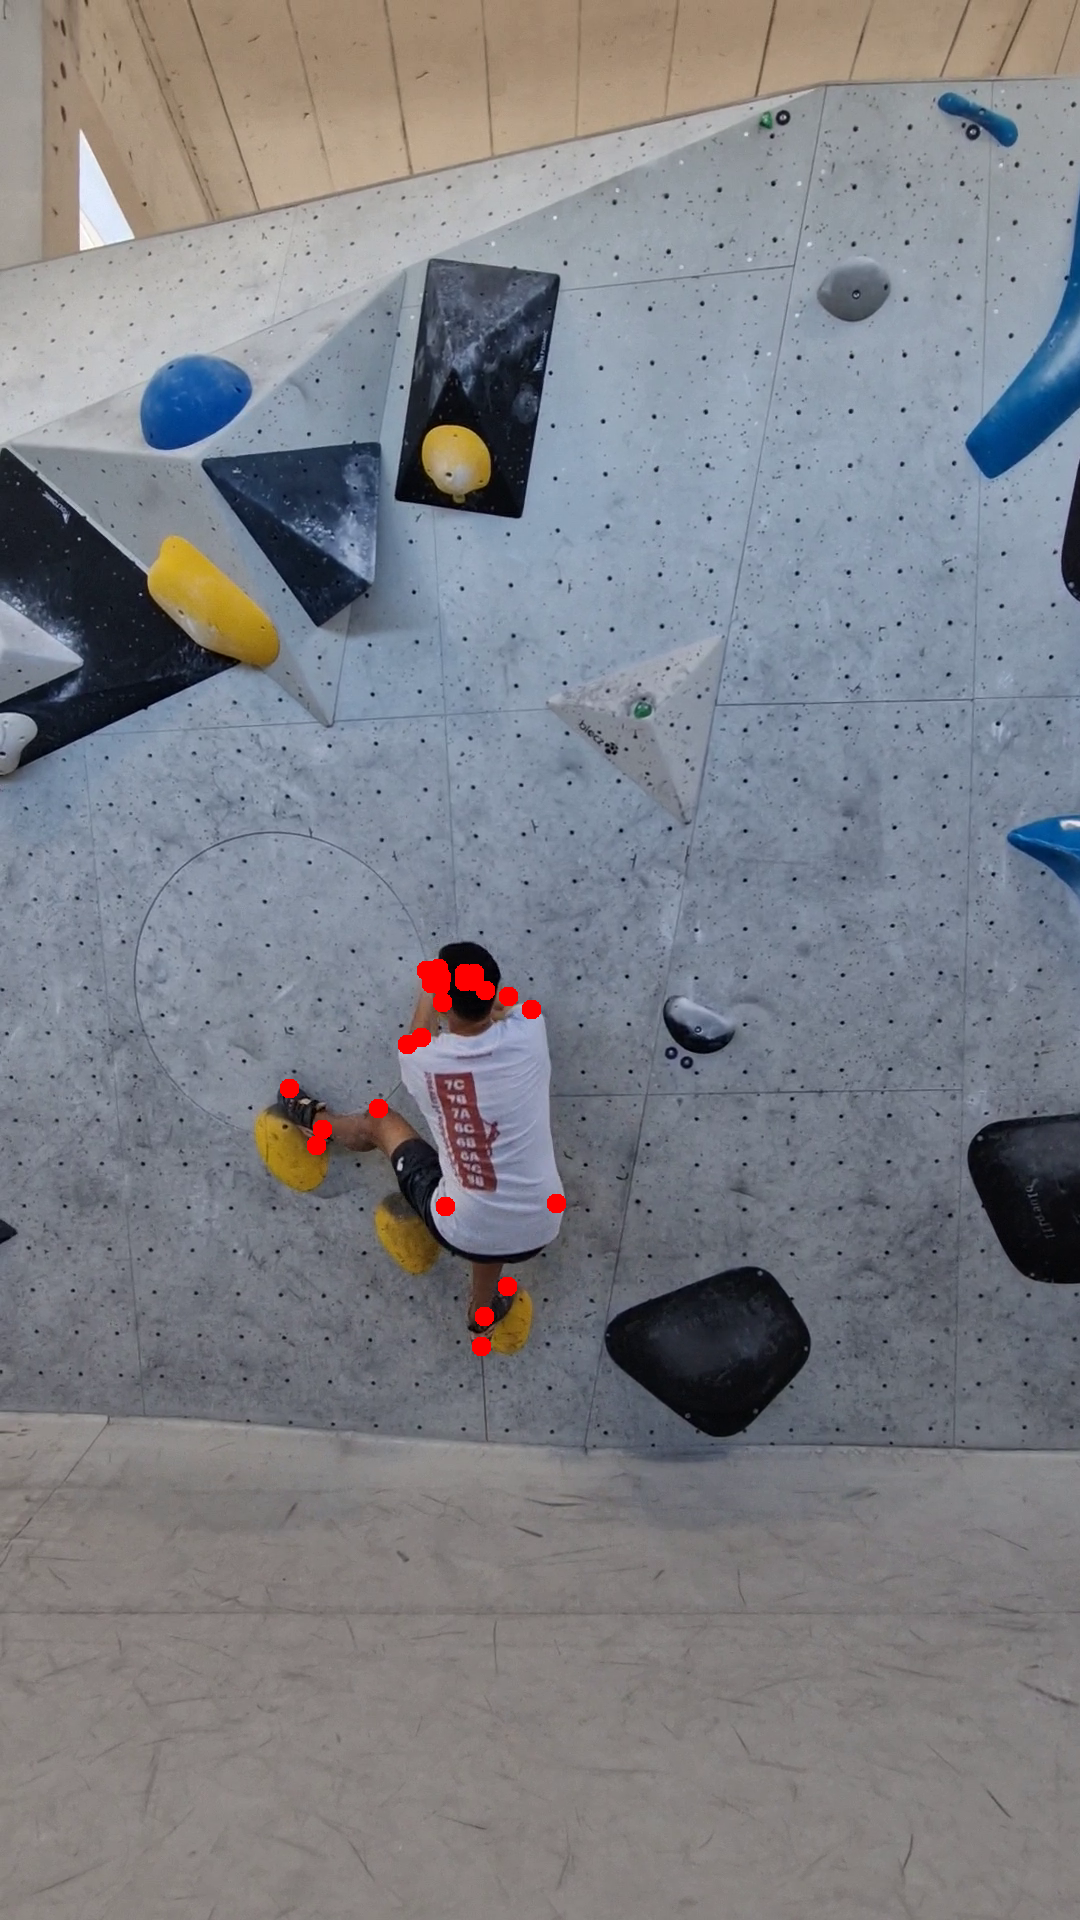
\includegraphics[width=\textwidth]{entities/CA_17.png}
        \caption{Frame 17}
    \end{subfigure}
    \begin{subfigure}{0.3\textwidth}
        \centering
        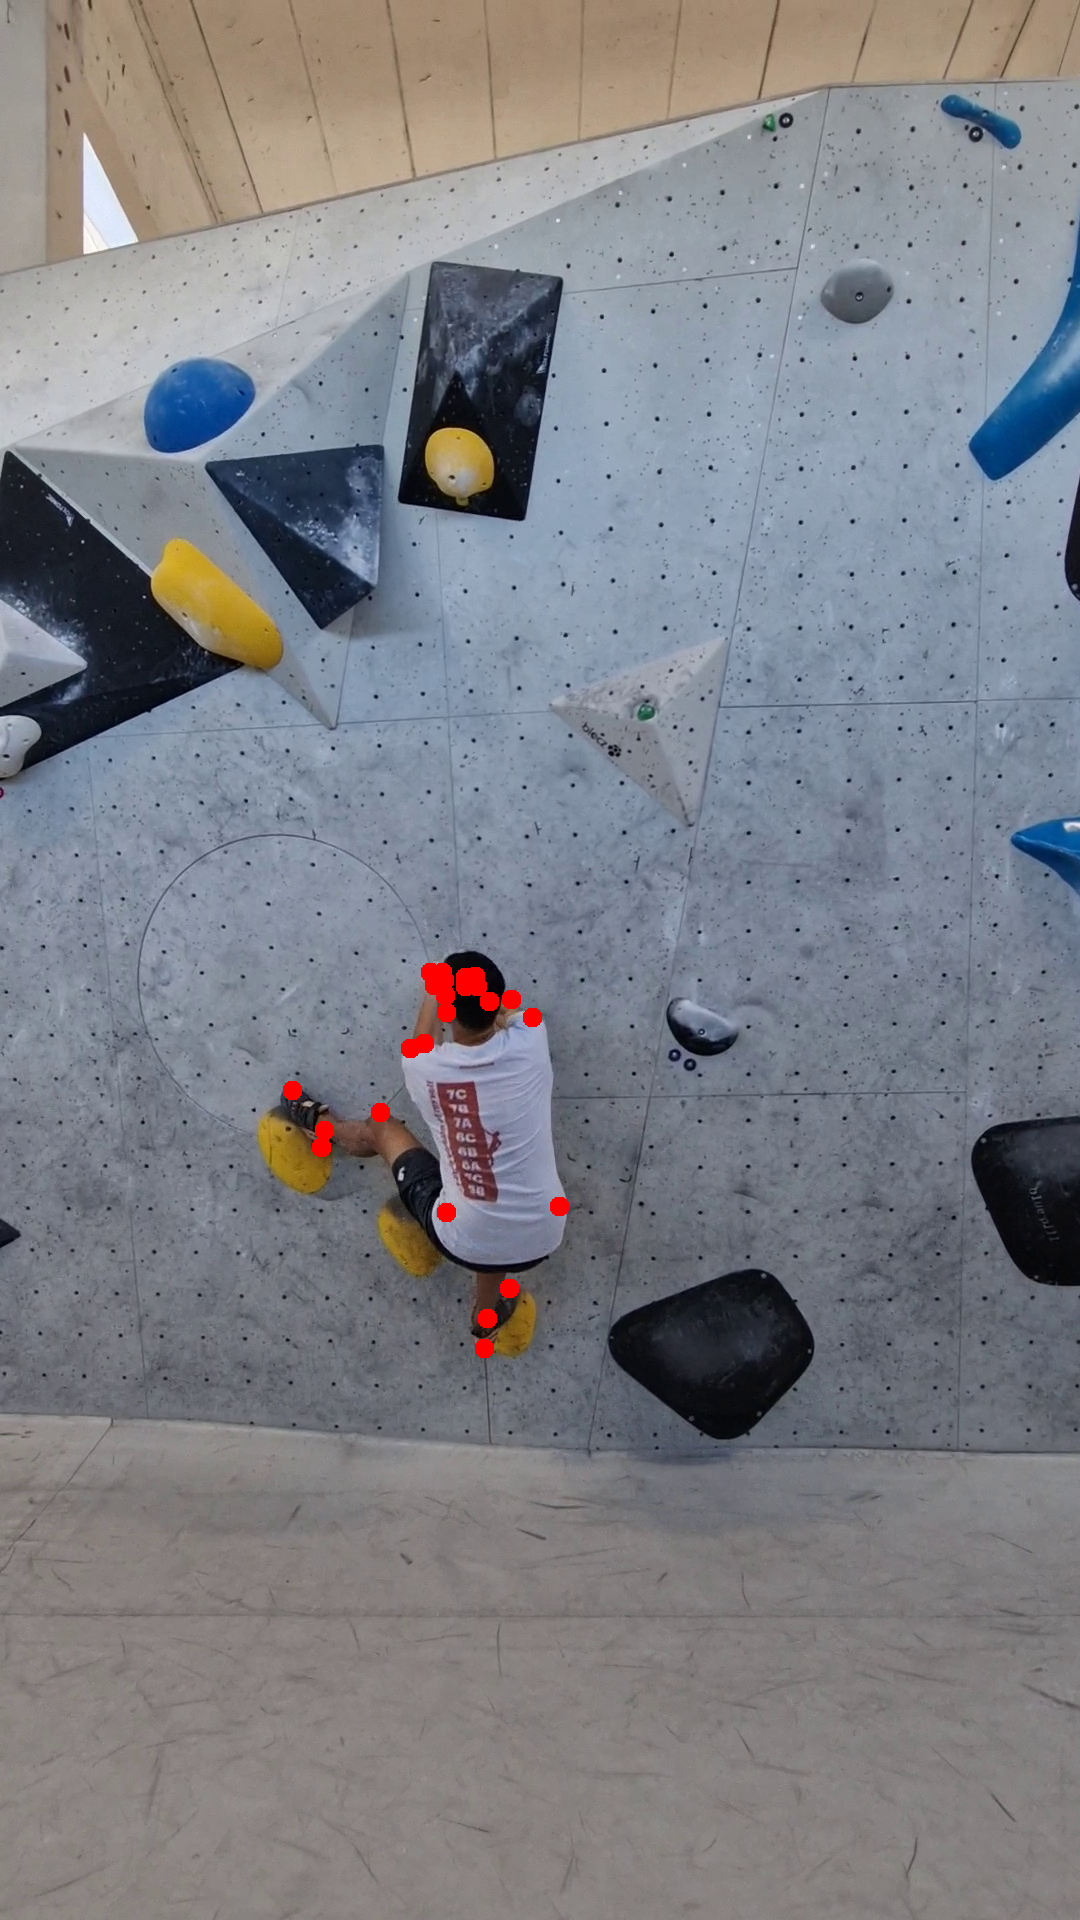
\includegraphics[width=\textwidth]{entities/CA_18.png}
        \caption{Frame 18}
    \end{subfigure}
    \begin{subfigure}{0.3\textwidth}
        \centering
        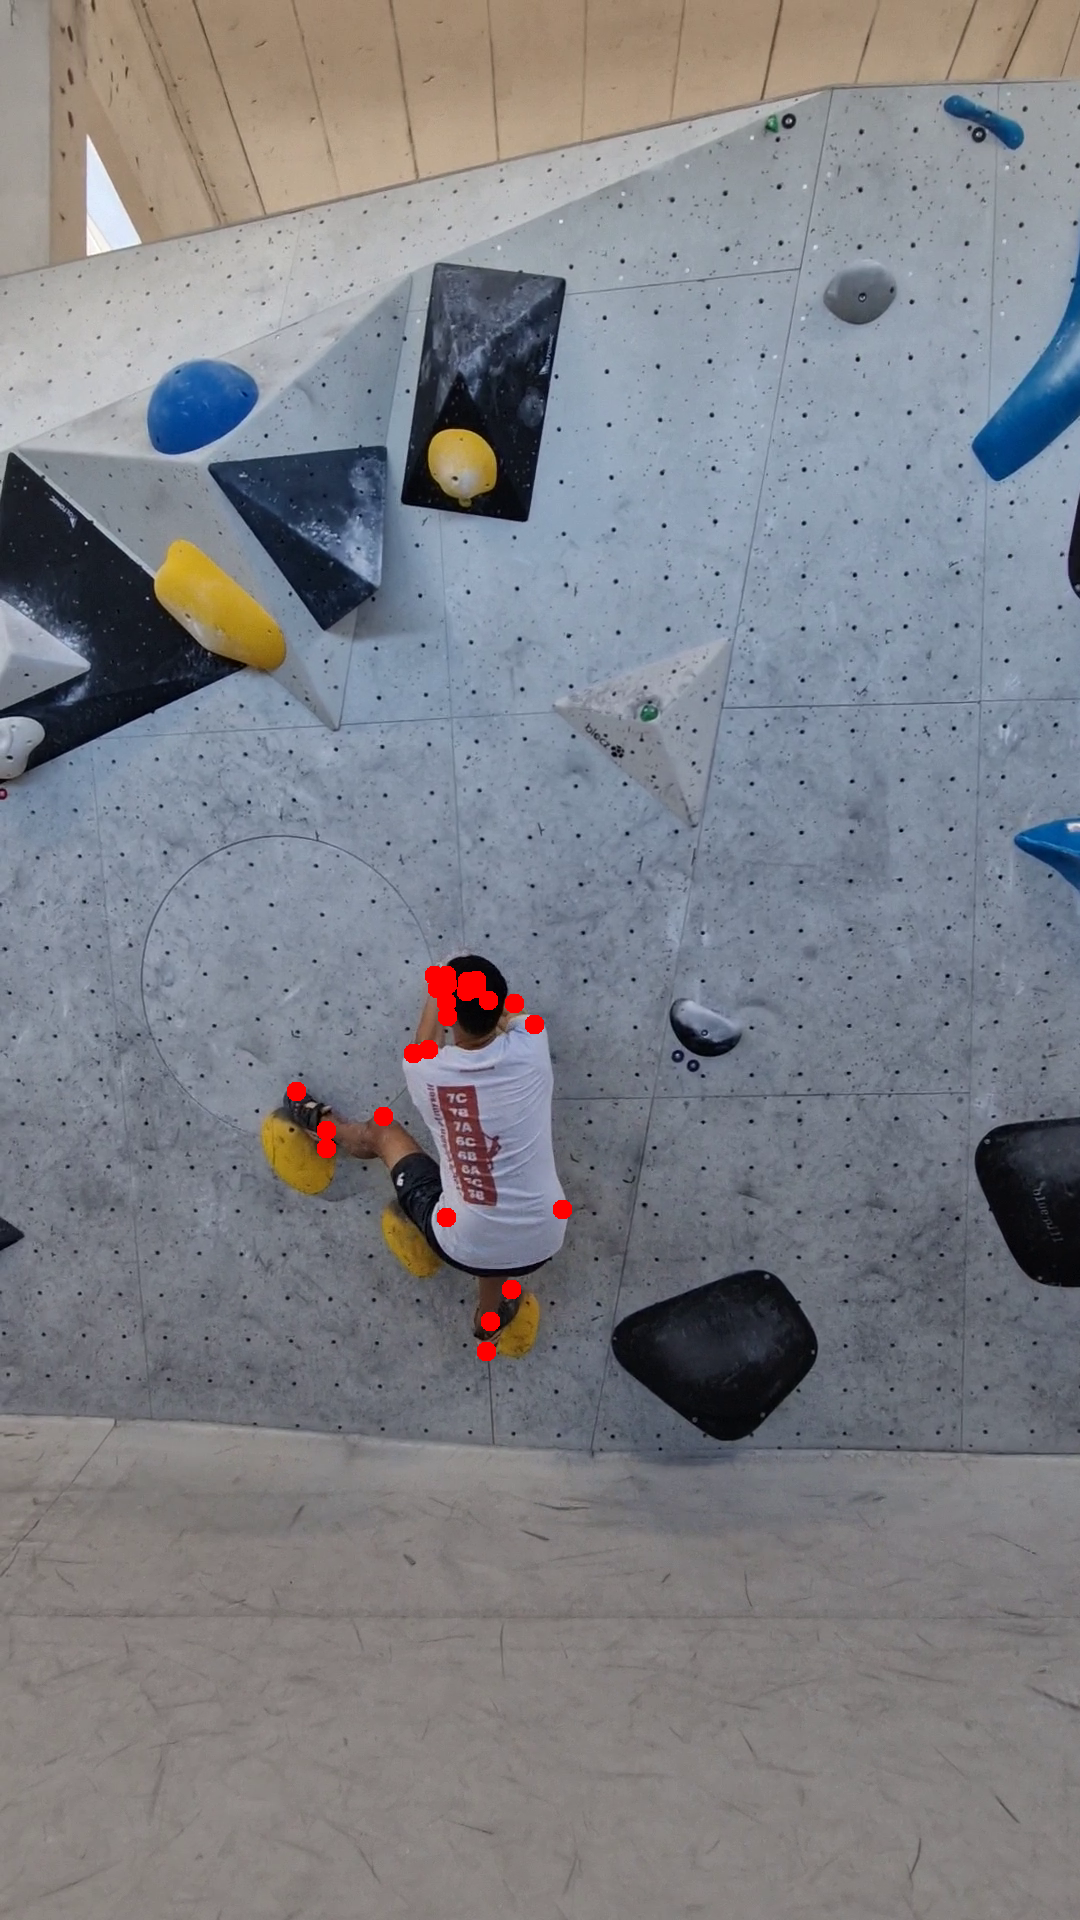
\includegraphics[width=\textwidth]{entities/CA_19.png}
        \caption{Frame 19}
    \end{subfigure}
    \begin{subfigure}{0.3\textwidth}
        \centering
        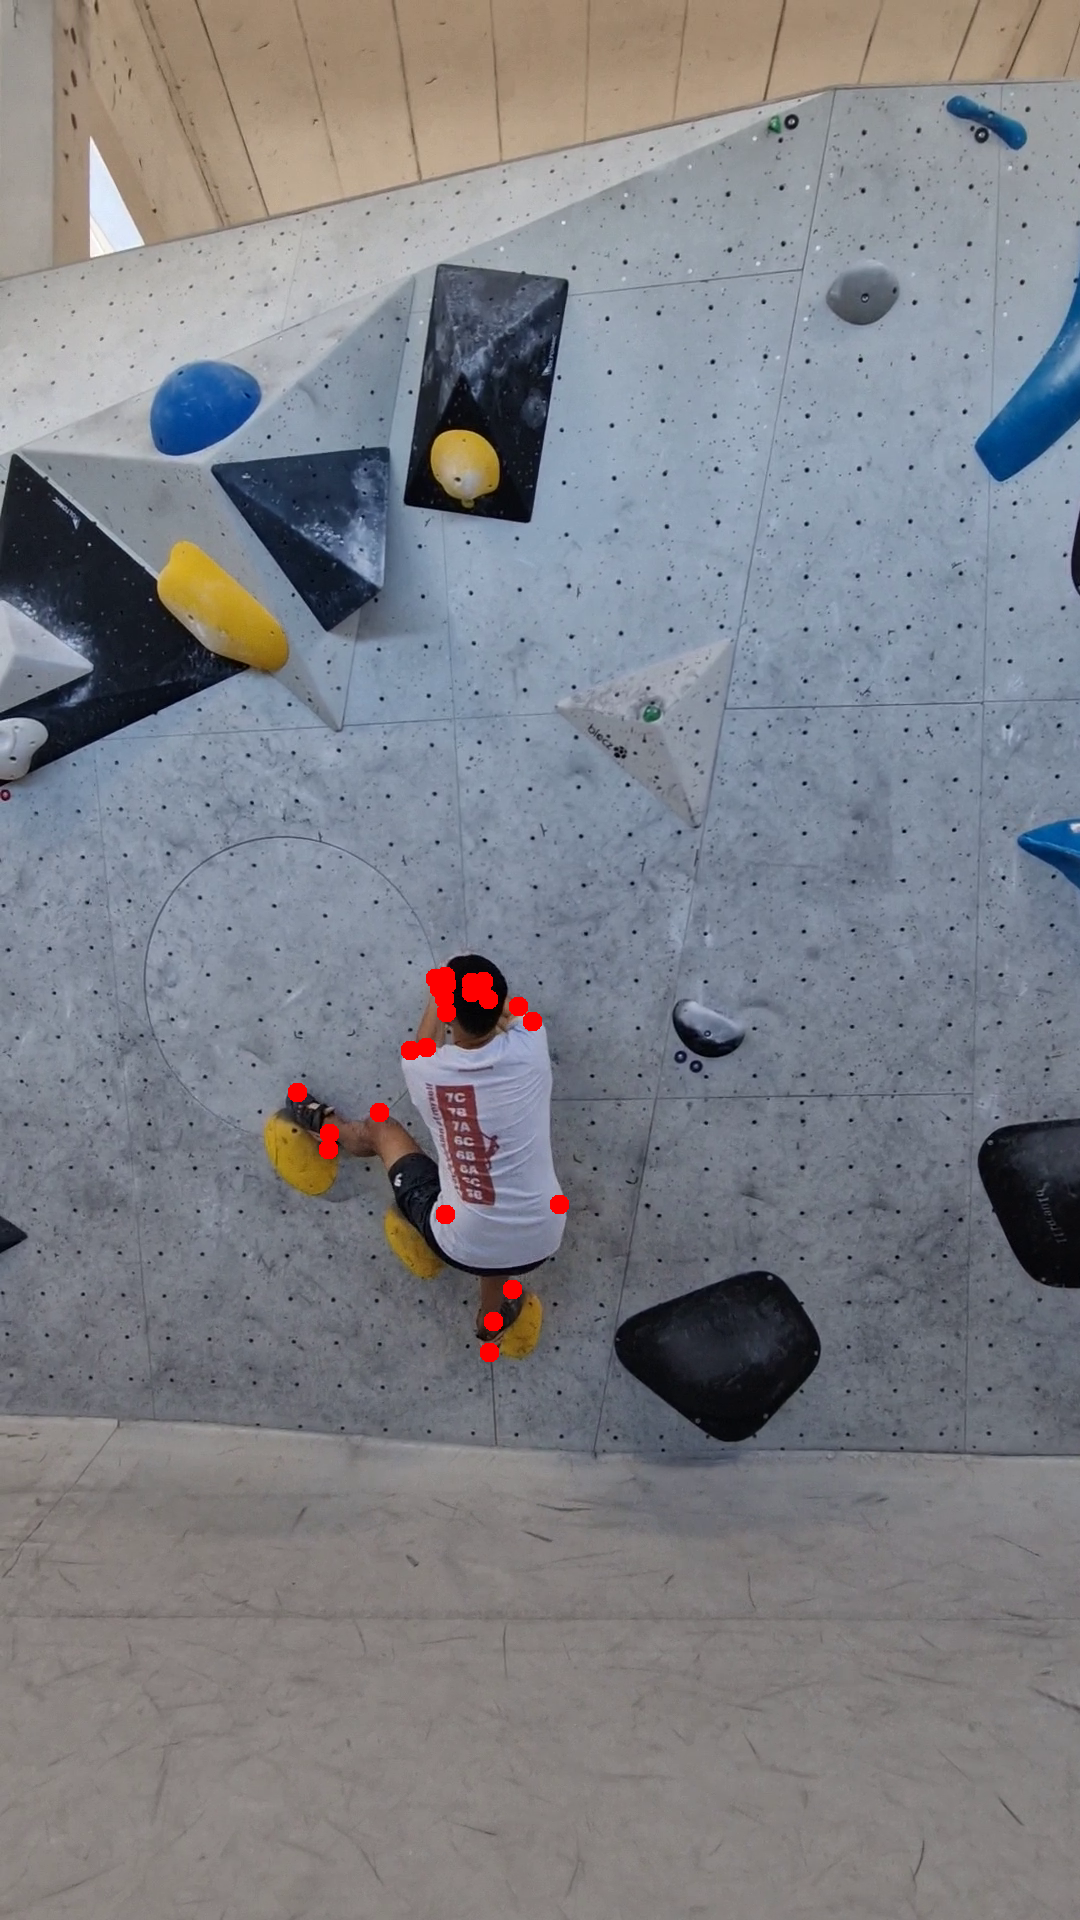
\includegraphics[width=\textwidth]{entities/CA_20.png}
        \caption{Frame 20}
    \end{subfigure}
    \begin{subfigure}{0.3\textwidth}
        \centering
        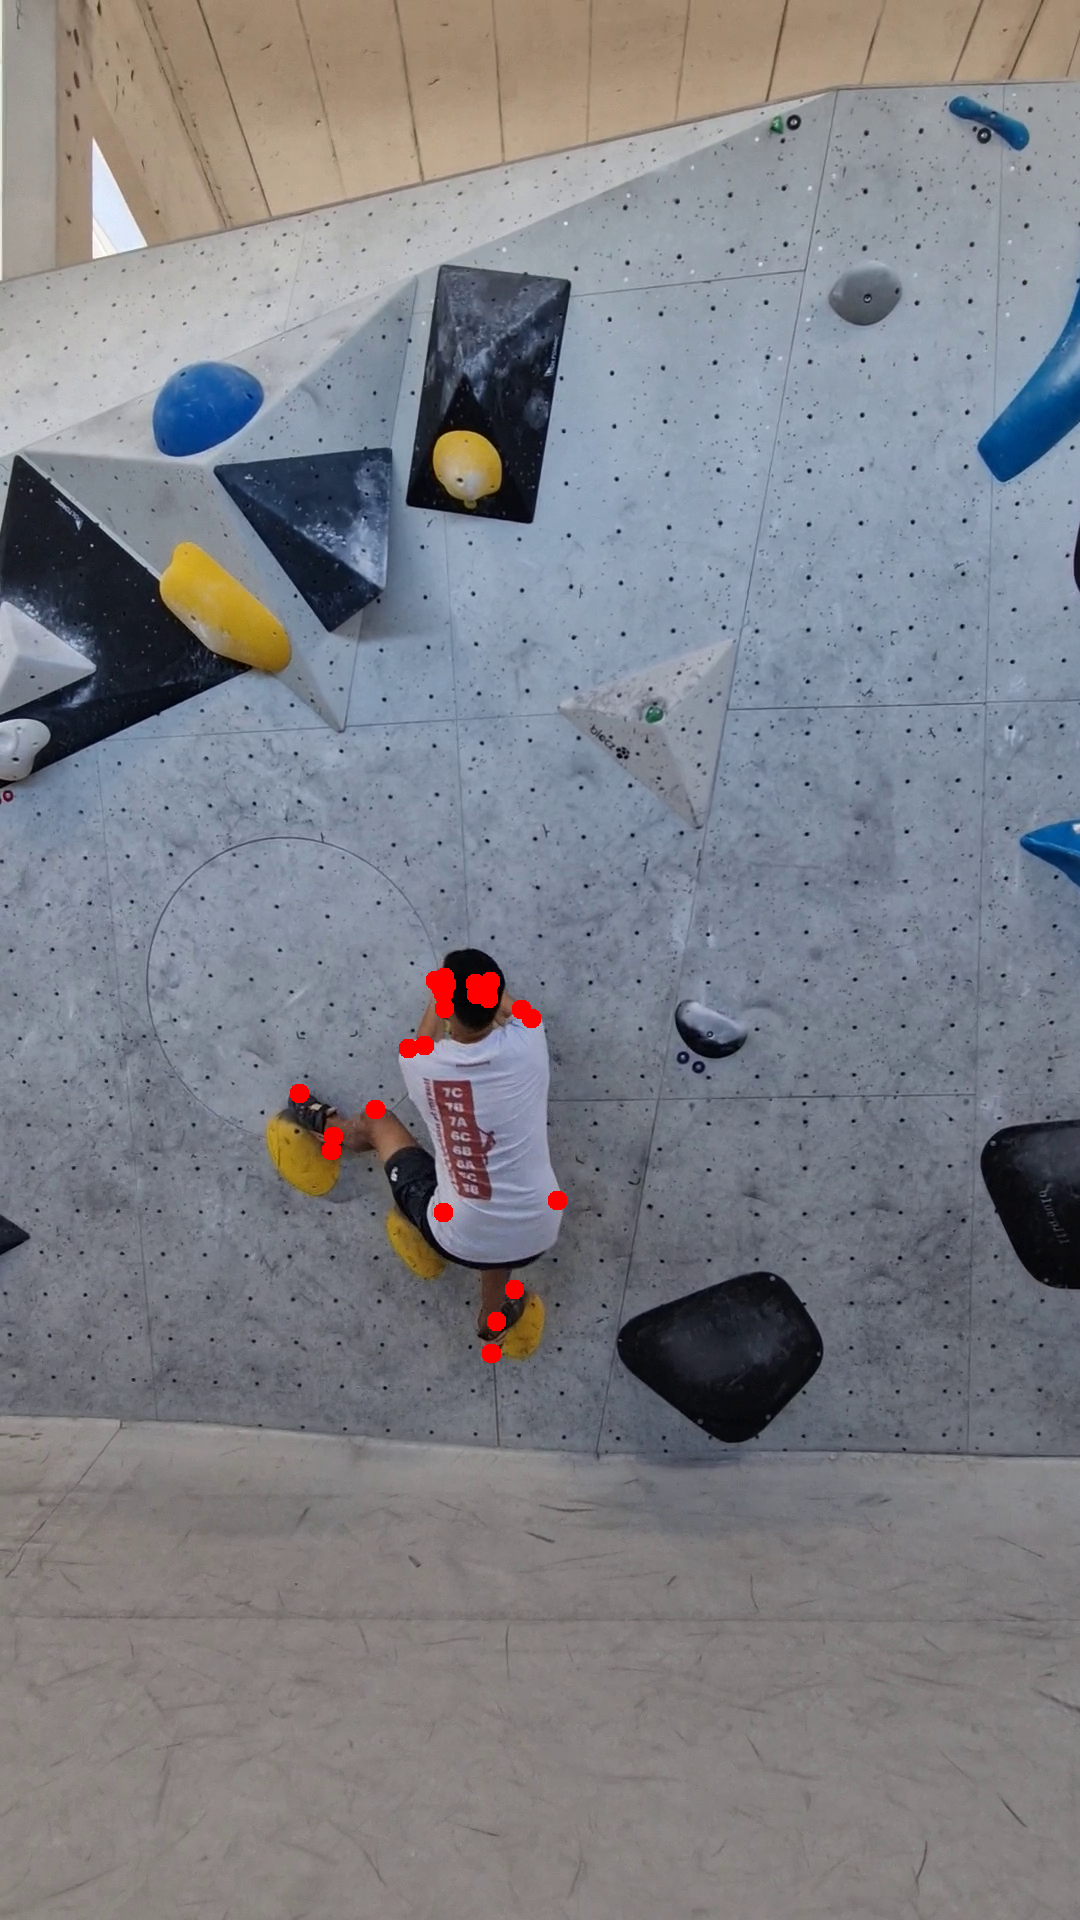
\includegraphics[width=\textwidth]{entities/CA_21.png}
        \caption{Frame 21}
    \end{subfigure}
    \caption{Example of five consecutive frames of a video from the ClimbAlong-dataset with the corresponding labels, where the actor holds his position for a while.}
    \label{fig:CA_dataset_static}
\end{figure}

\begin{figure}[htbp]
    \centering
    \begin{subfigure}{0.3\textwidth}
        \centering
        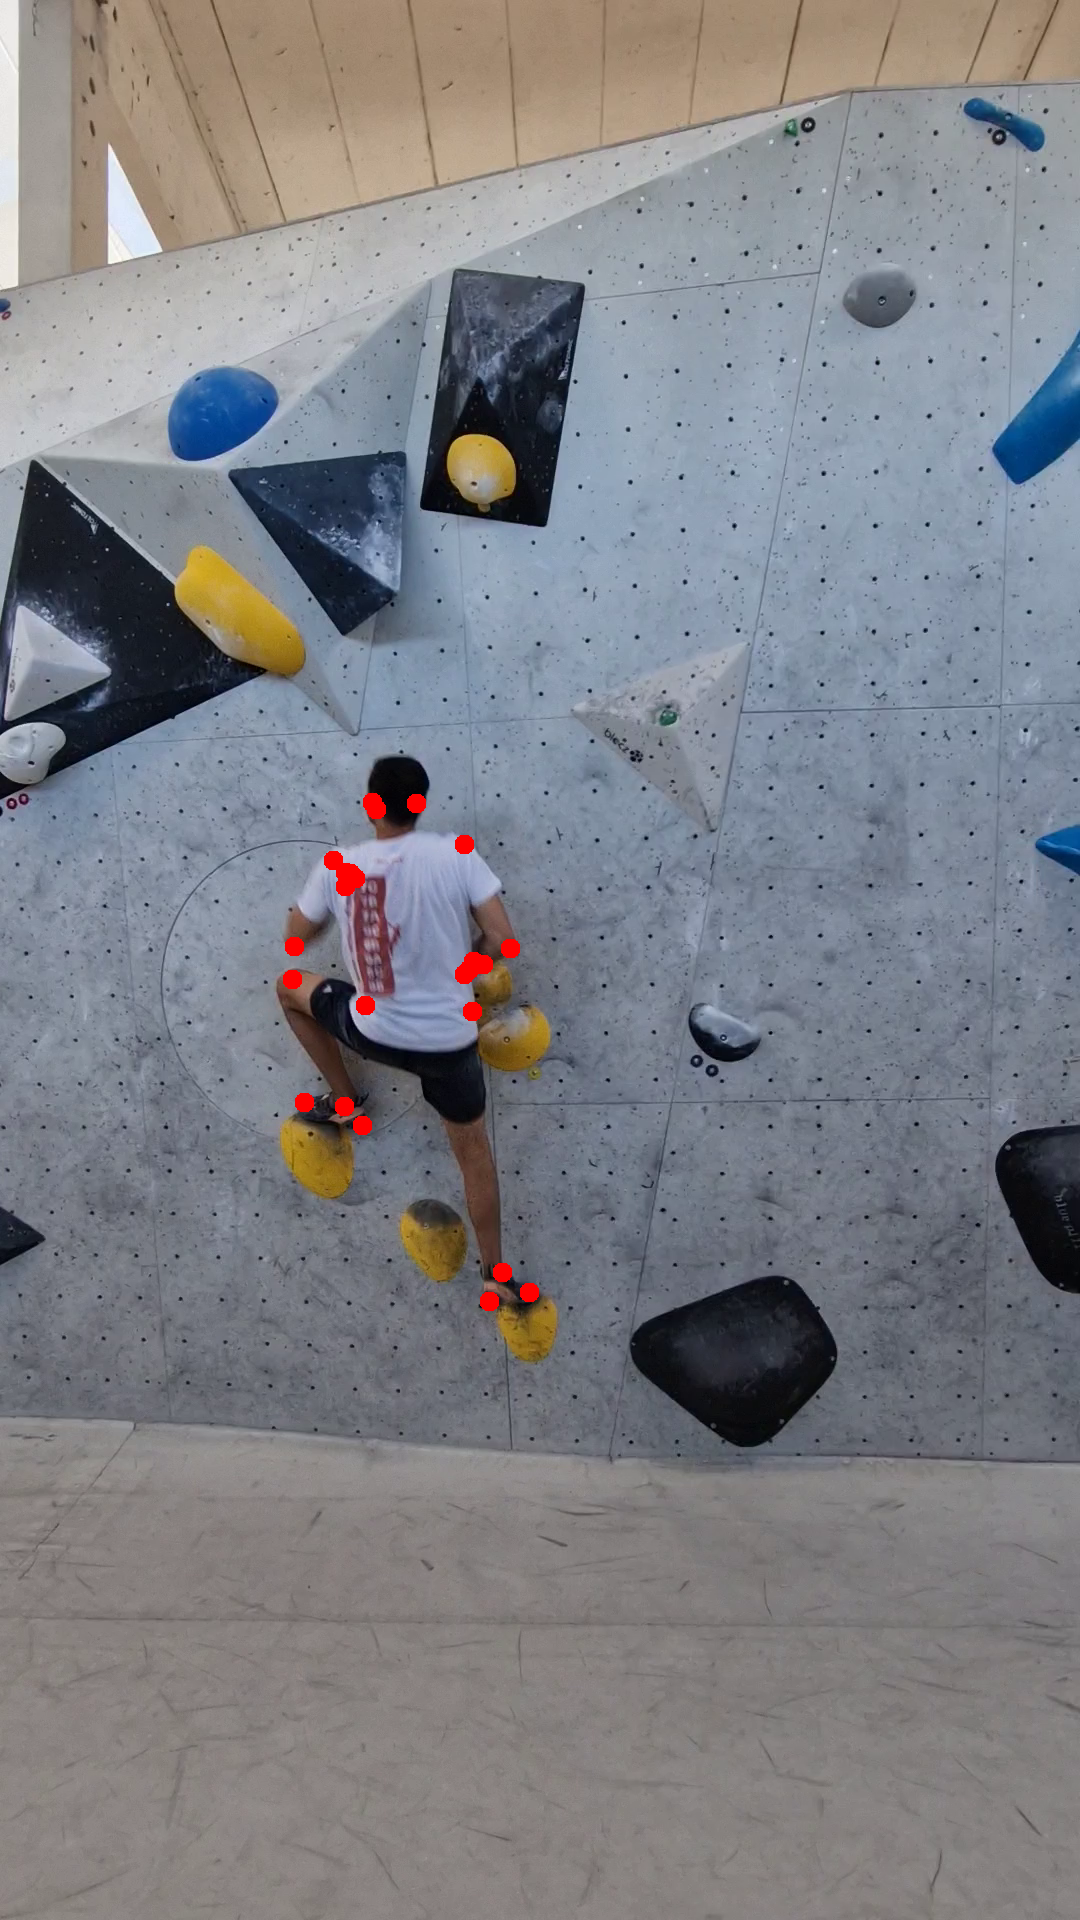
\includegraphics[width=\textwidth]{entities/CA_31.png}
        \caption{Frame 31}
    \end{subfigure}
    \begin{subfigure}{0.3\textwidth}
        \centering
        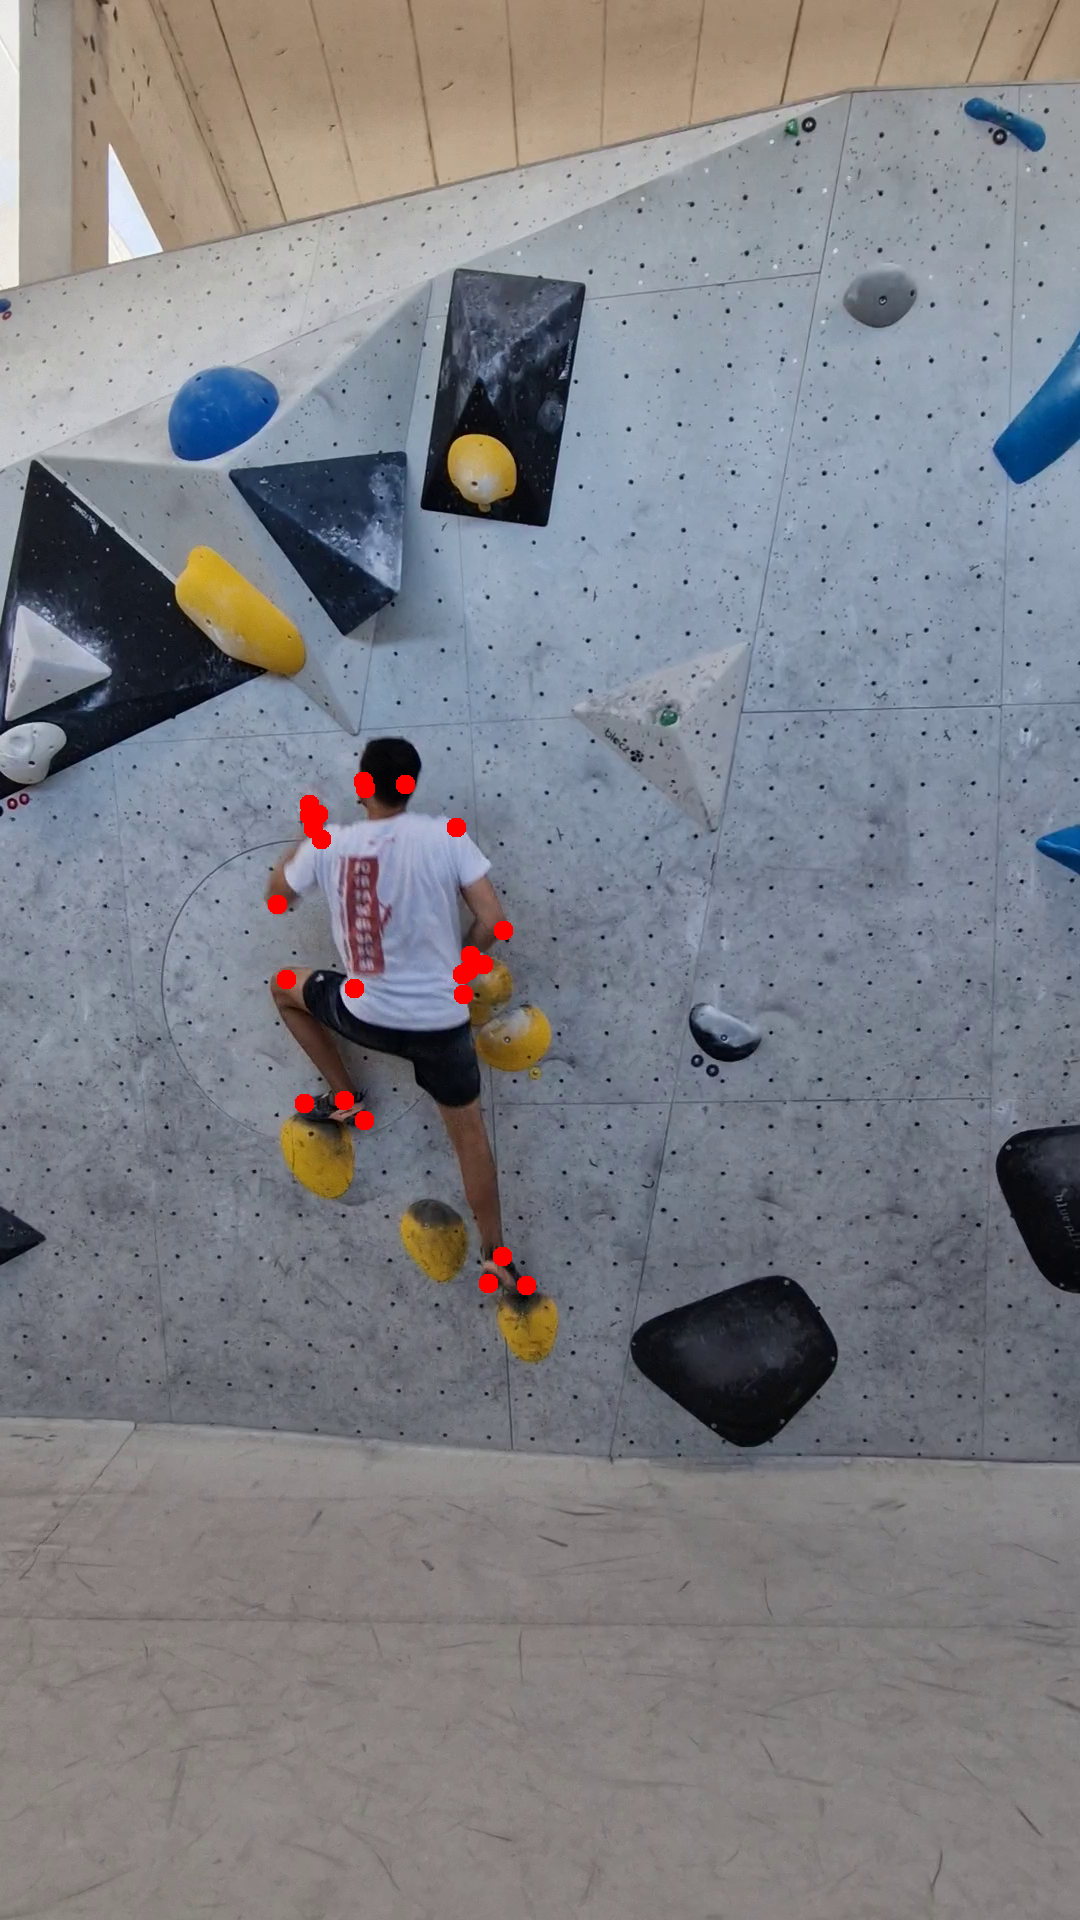
\includegraphics[width=\textwidth]{entities/CA_32.png}
        \caption{Frame 32}
    \end{subfigure}
    \begin{subfigure}{0.3\textwidth}
        \centering
        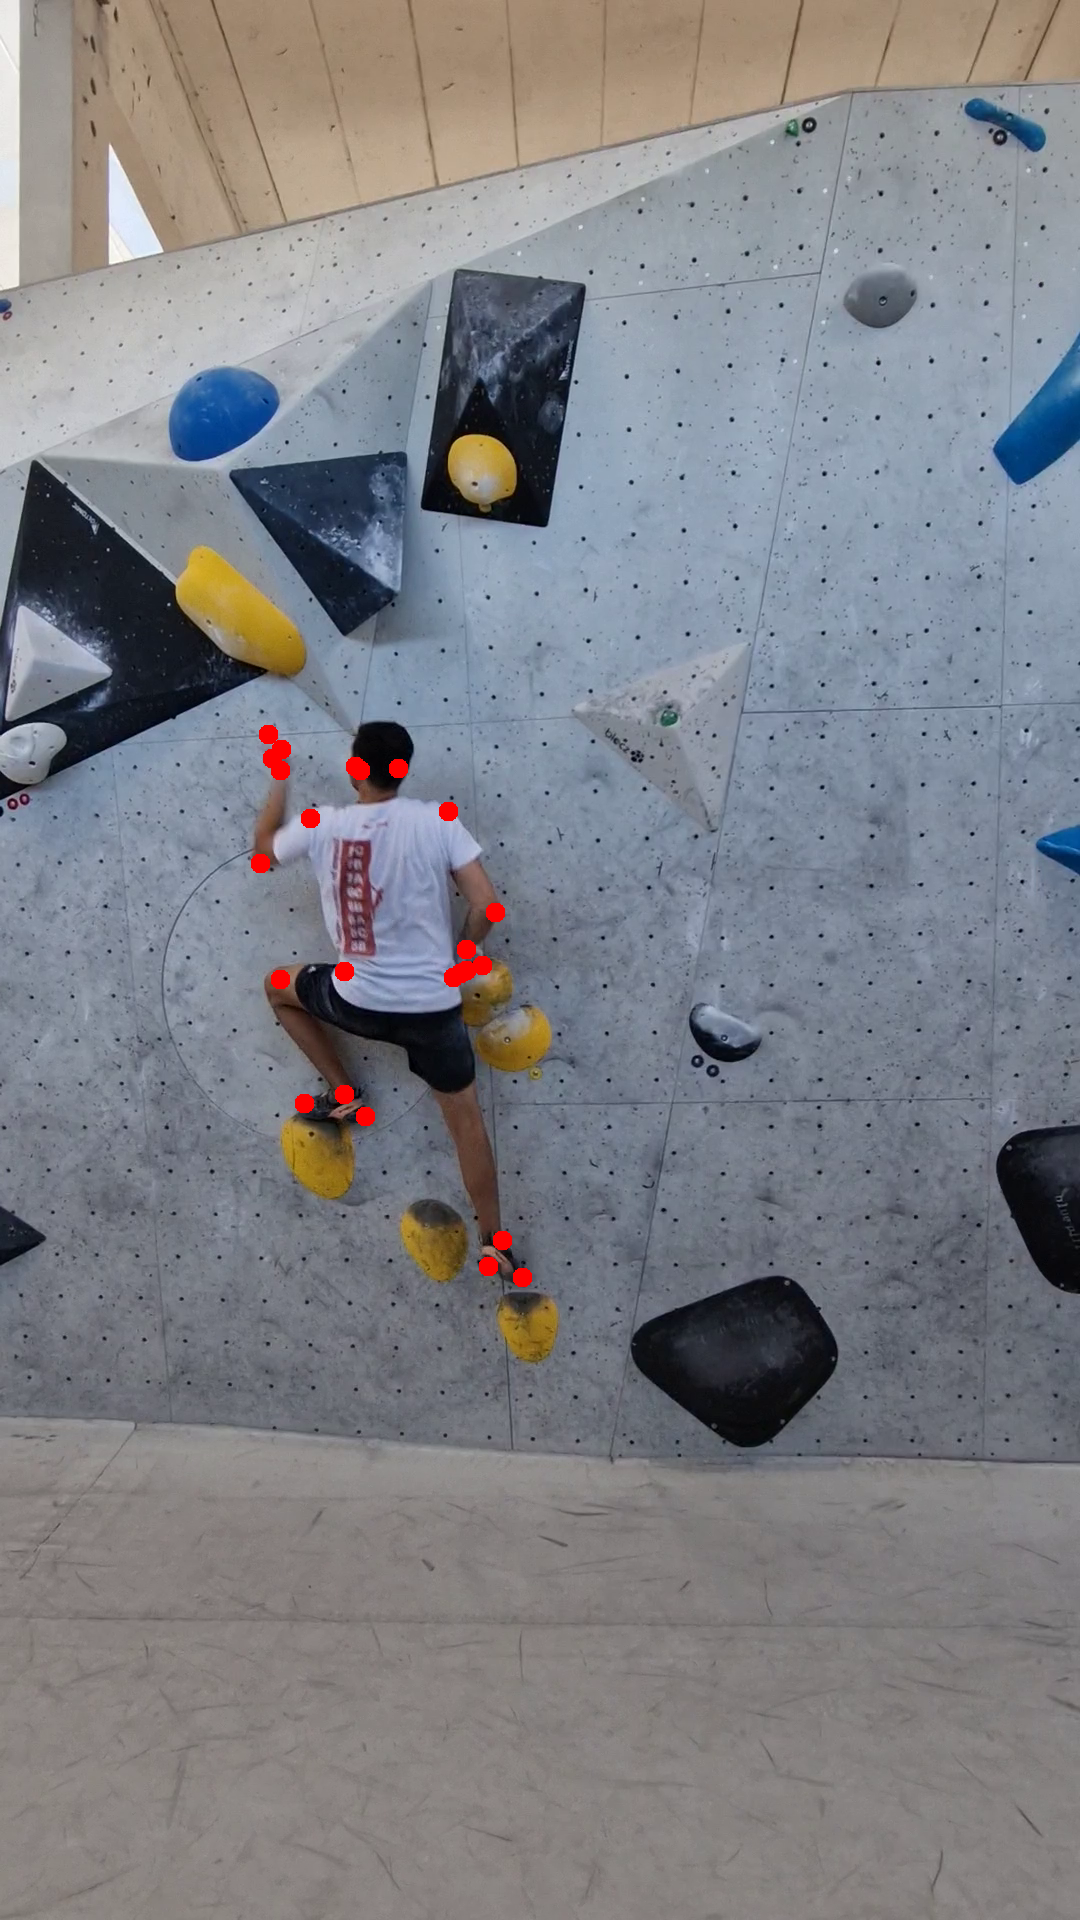
\includegraphics[width=\textwidth]{entities/CA_33.png}
        \caption{Frame 33}
    \end{subfigure}
    \begin{subfigure}{0.3\textwidth}
        \centering
        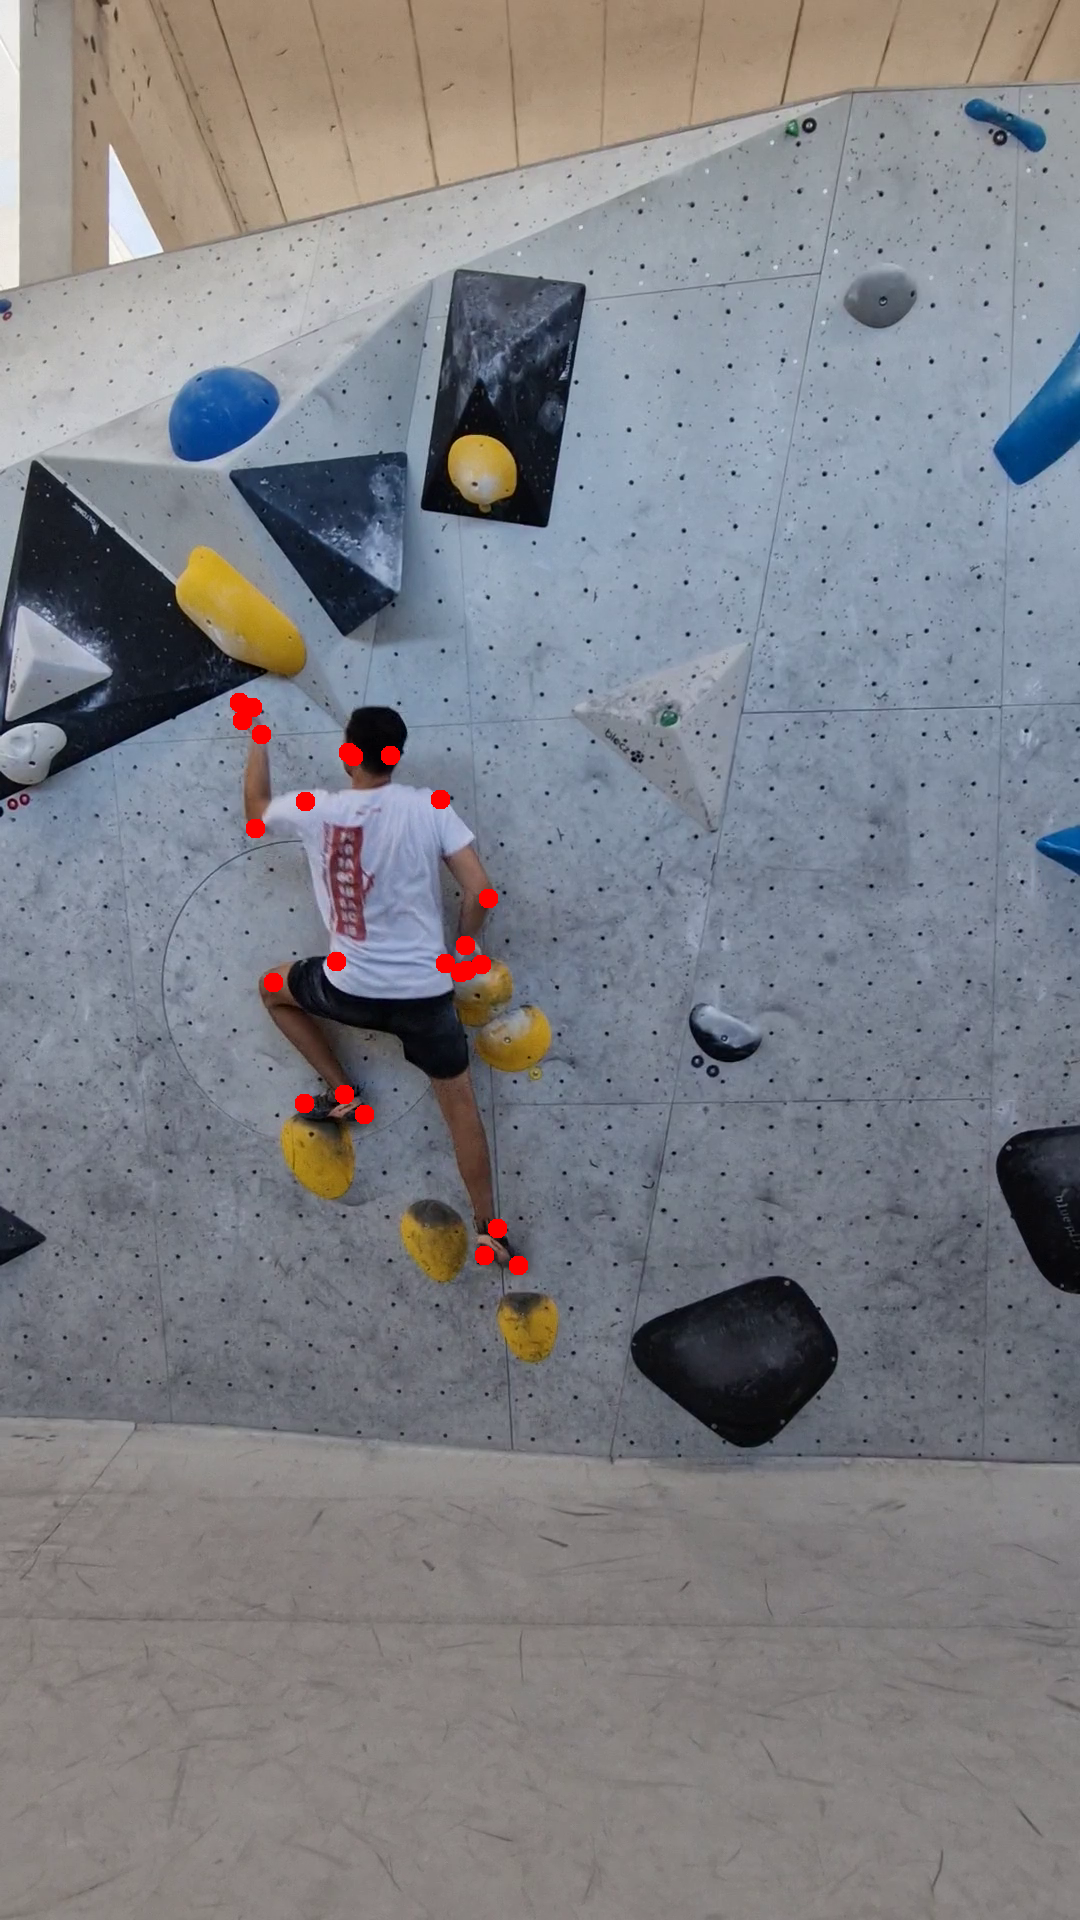
\includegraphics[width=\textwidth]{entities/CA_34.png}
        \caption{Frame 34}
    \end{subfigure}
    \begin{subfigure}{0.3\textwidth}
        \centering
        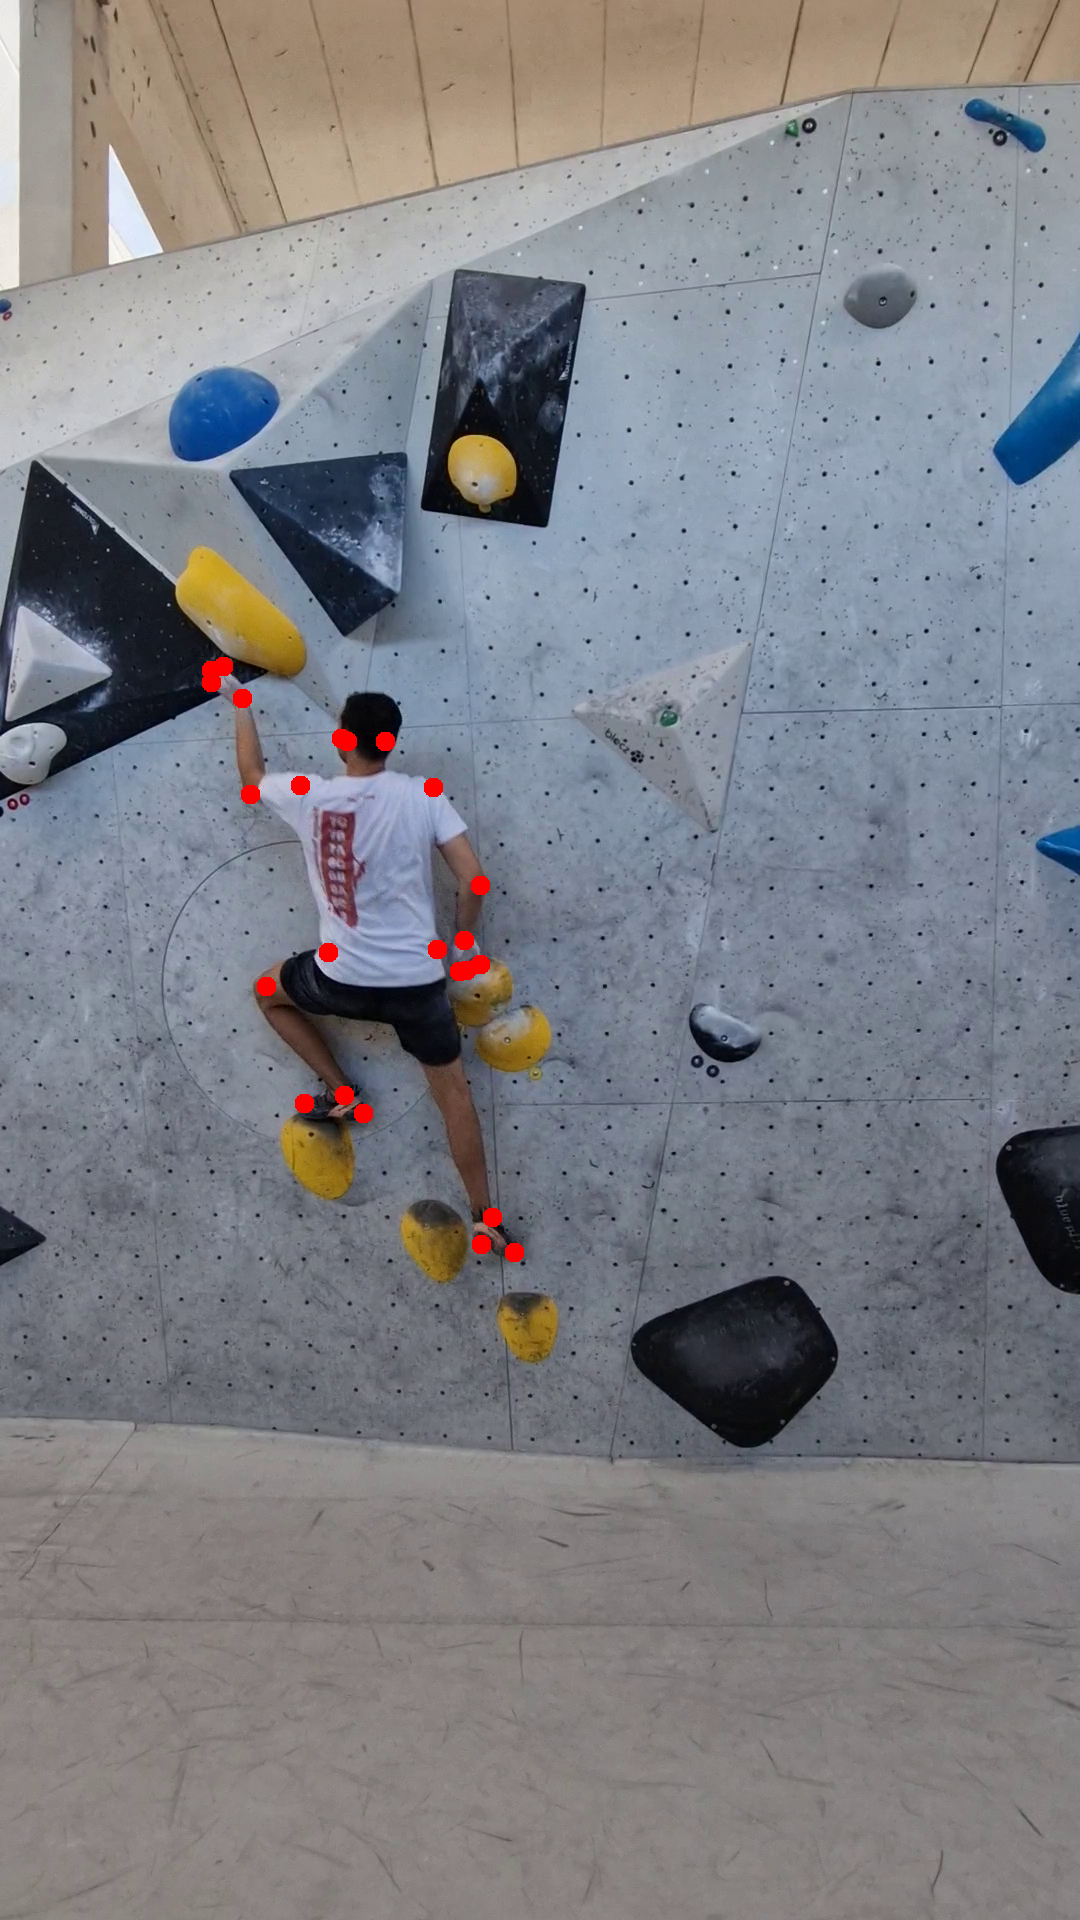
\includegraphics[width=\textwidth]{entities/CA_35.png}
        \caption{Frame 35}
    \end{subfigure}

    \caption{Example of five consecutive frames of a video from the ClimbAlong-dataset with the corresponding labels, where the actor performs a quick movement.}
    \label{fig:CA_dataset_quick}
\end{figure}

As the aim of our models is to perform well on climbers, we will be using some annotated data of climbers. For this, ClimbAlong ApS has developed a dataset that we will be using. The dataset consists of videos of various climbers on bouldering walls, where each video contains just a single climber. Figure \ref{fig:CA_dataset_static} and \ref{fig:CA_dataset_quick} illustrates two windows of five consecutive frames of a single video from the ClimbAlong dataset. As shown in the figures, the videos in the dataset contains both static positions, where the climber holds a position for a while, as well as quick movemeents.
\\
\\
The ClimbAlong-dataset is split into two subsets. The first subset consists of $31$ fully annotated videos, where each annotation consists of $25$ keypoints. The second subset consists of $110$ fully annotated videos, where each annotation consists of $17$ keypoints. The two subsets have $13$ overlapping videos.
\\
\\
Each videos is filmed in portrait mode with a resolution of $1080 \times 1920$ and $30$ frames per second. Table \ref{tab:keypoints} gives an overview of which keypoints are annotated in the two subsets. 

\subsection{The BRACE Dataset}
\begin{figure}[htbp]
    \centering
    \begin{subfigure}{0.5\textwidth}
        \centering
        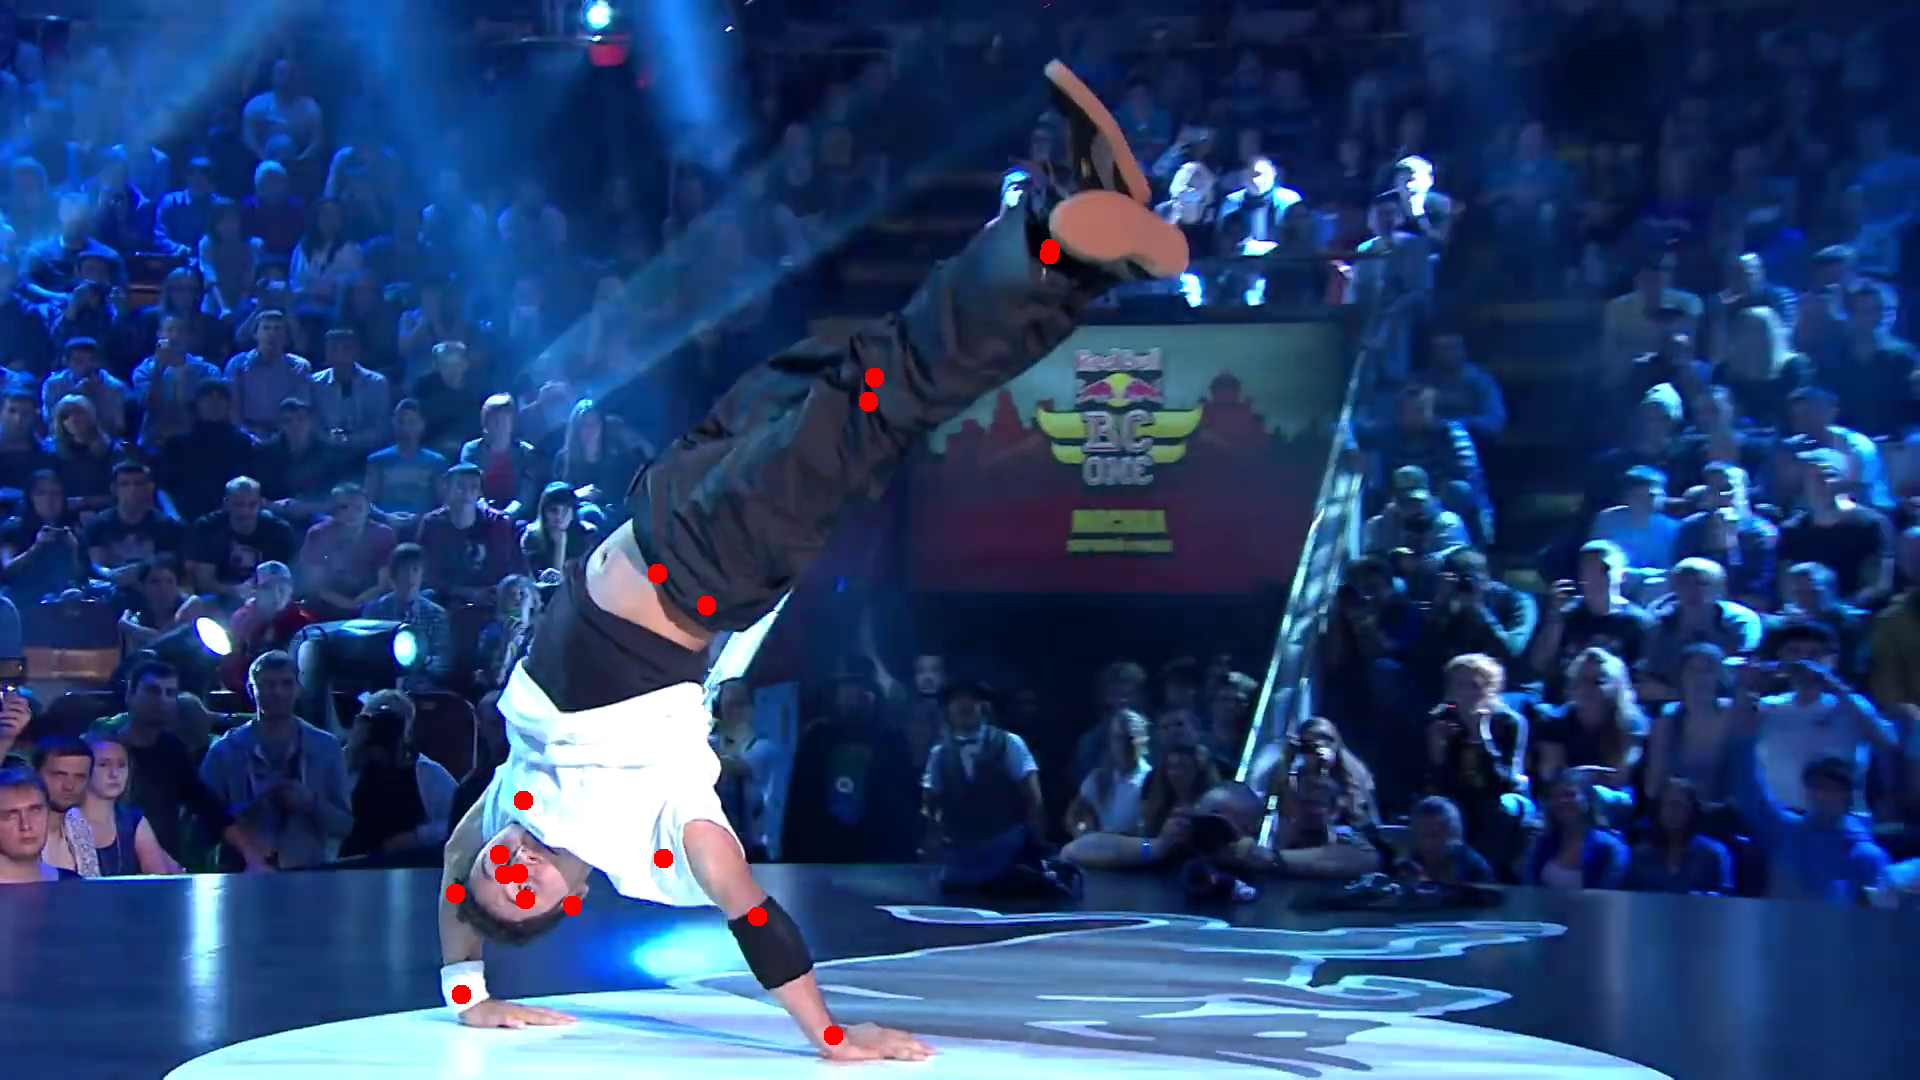
\includegraphics[width=\textwidth]{entities/BRACE_2450.png}
        \caption{Frame 2450}
    \end{subfigure}
    \begin{subfigure}{0.5\textwidth}
        \centering
        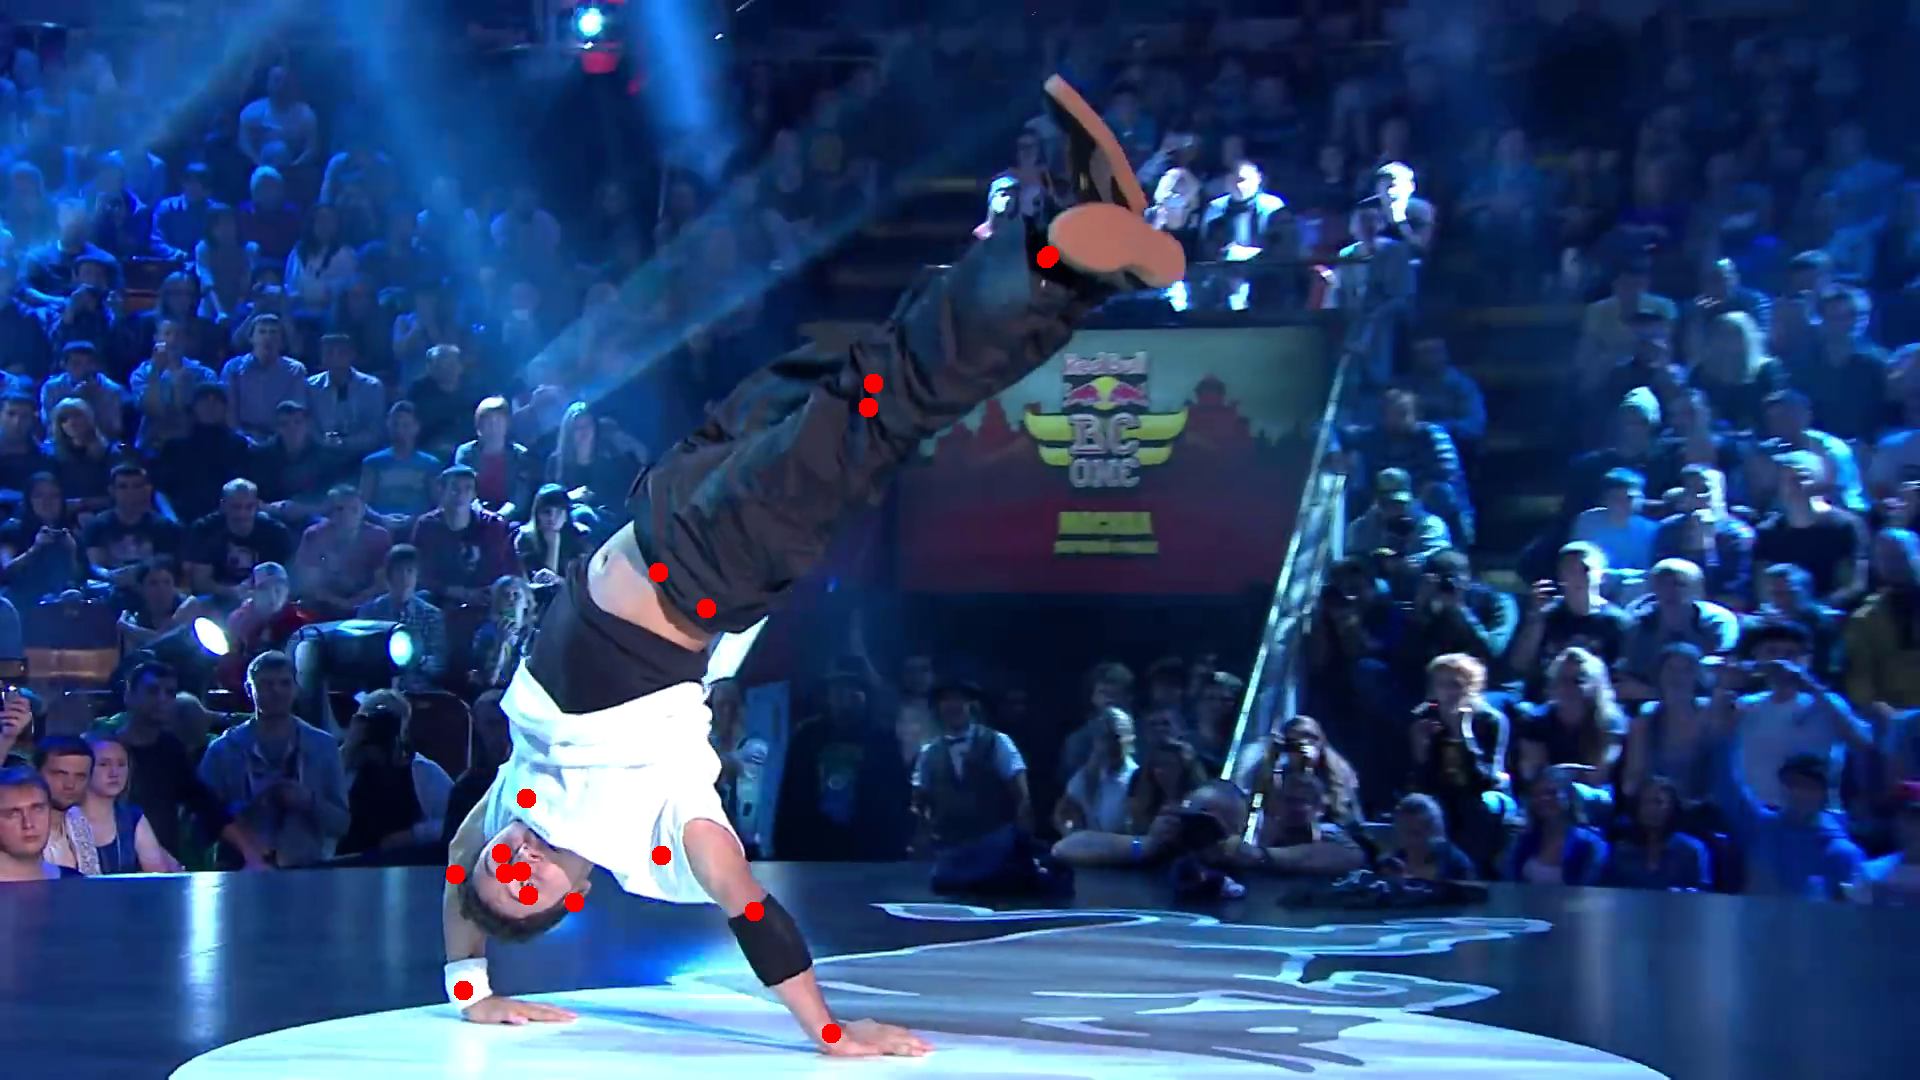
\includegraphics[width=\textwidth]{entities/BRACE_2451.png}
        \caption{Frame 2451}
    \end{subfigure}
    \begin{subfigure}{0.5\textwidth}
        \centering
        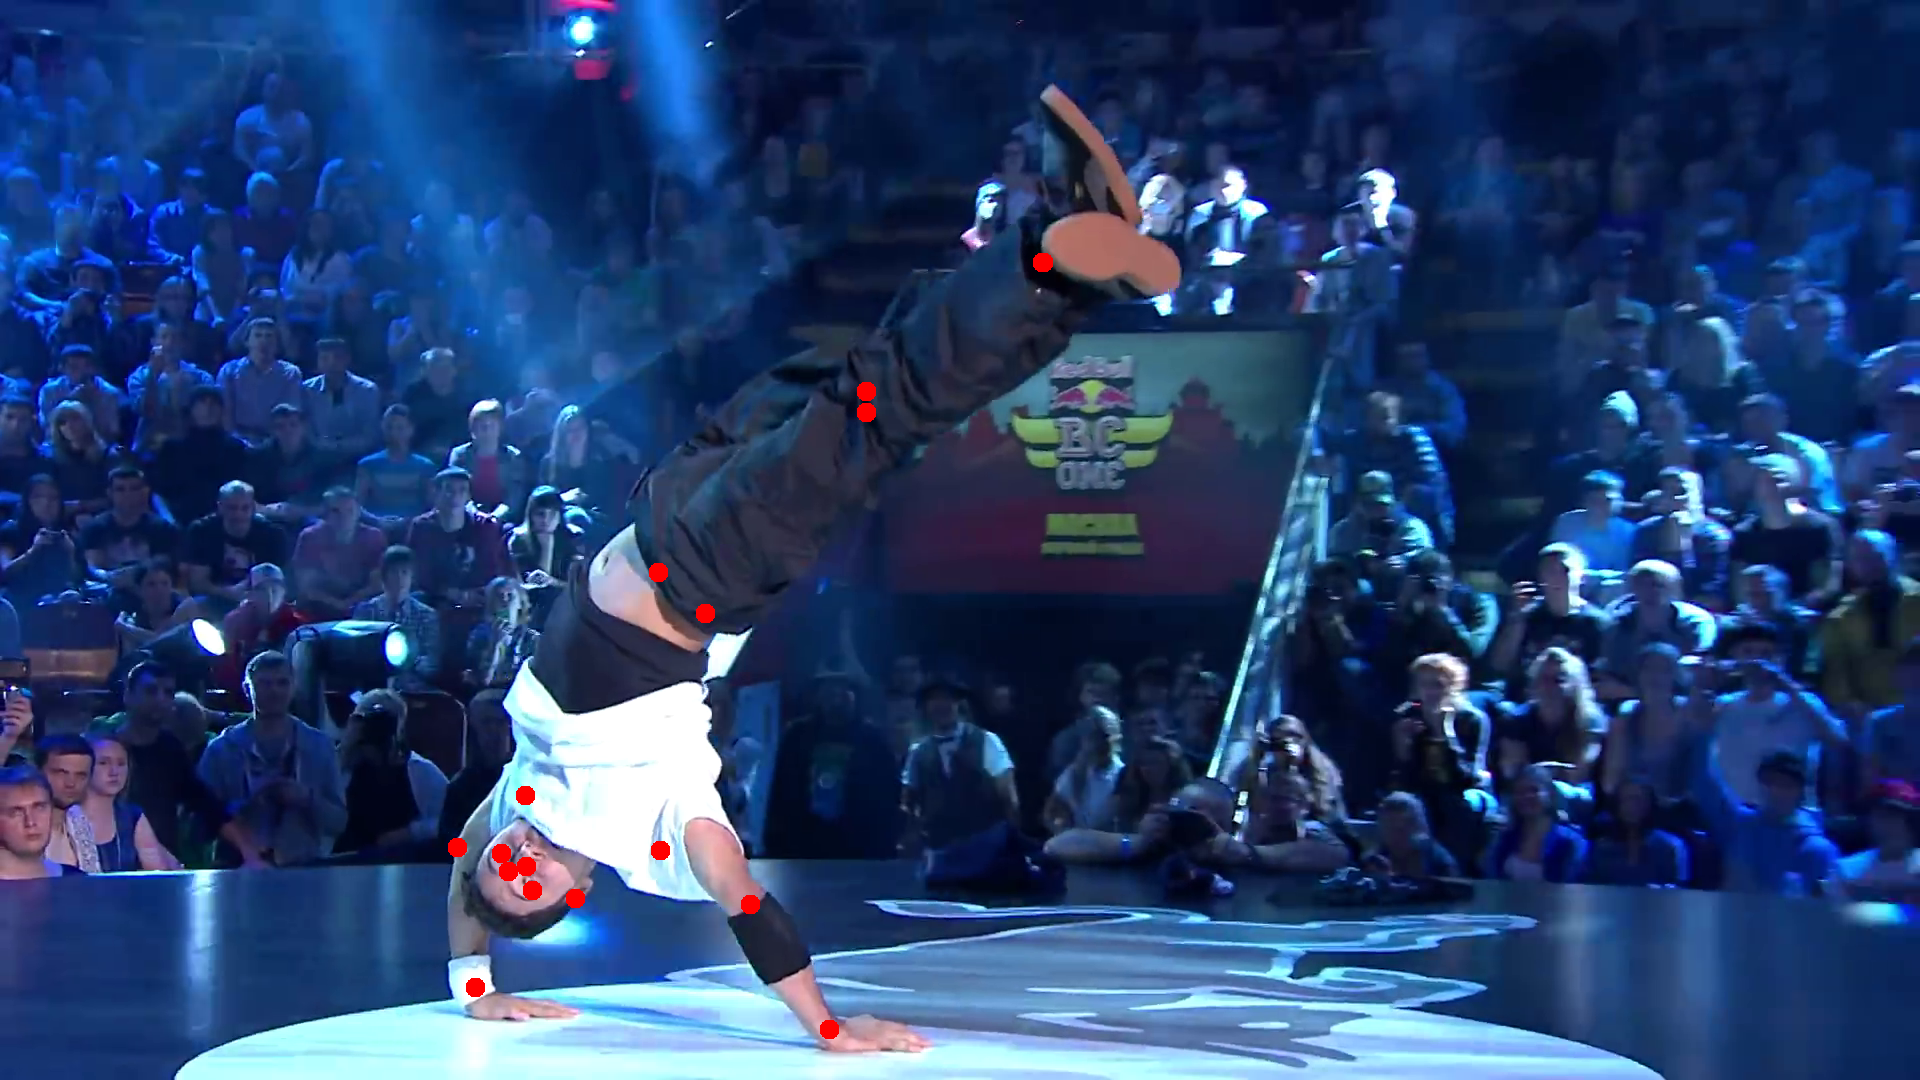
\includegraphics[width=\textwidth]{entities/BRACE_2452.png}
        \caption{Frame 2452}
    \end{subfigure}
    \begin{subfigure}{0.5\textwidth}
        \centering
        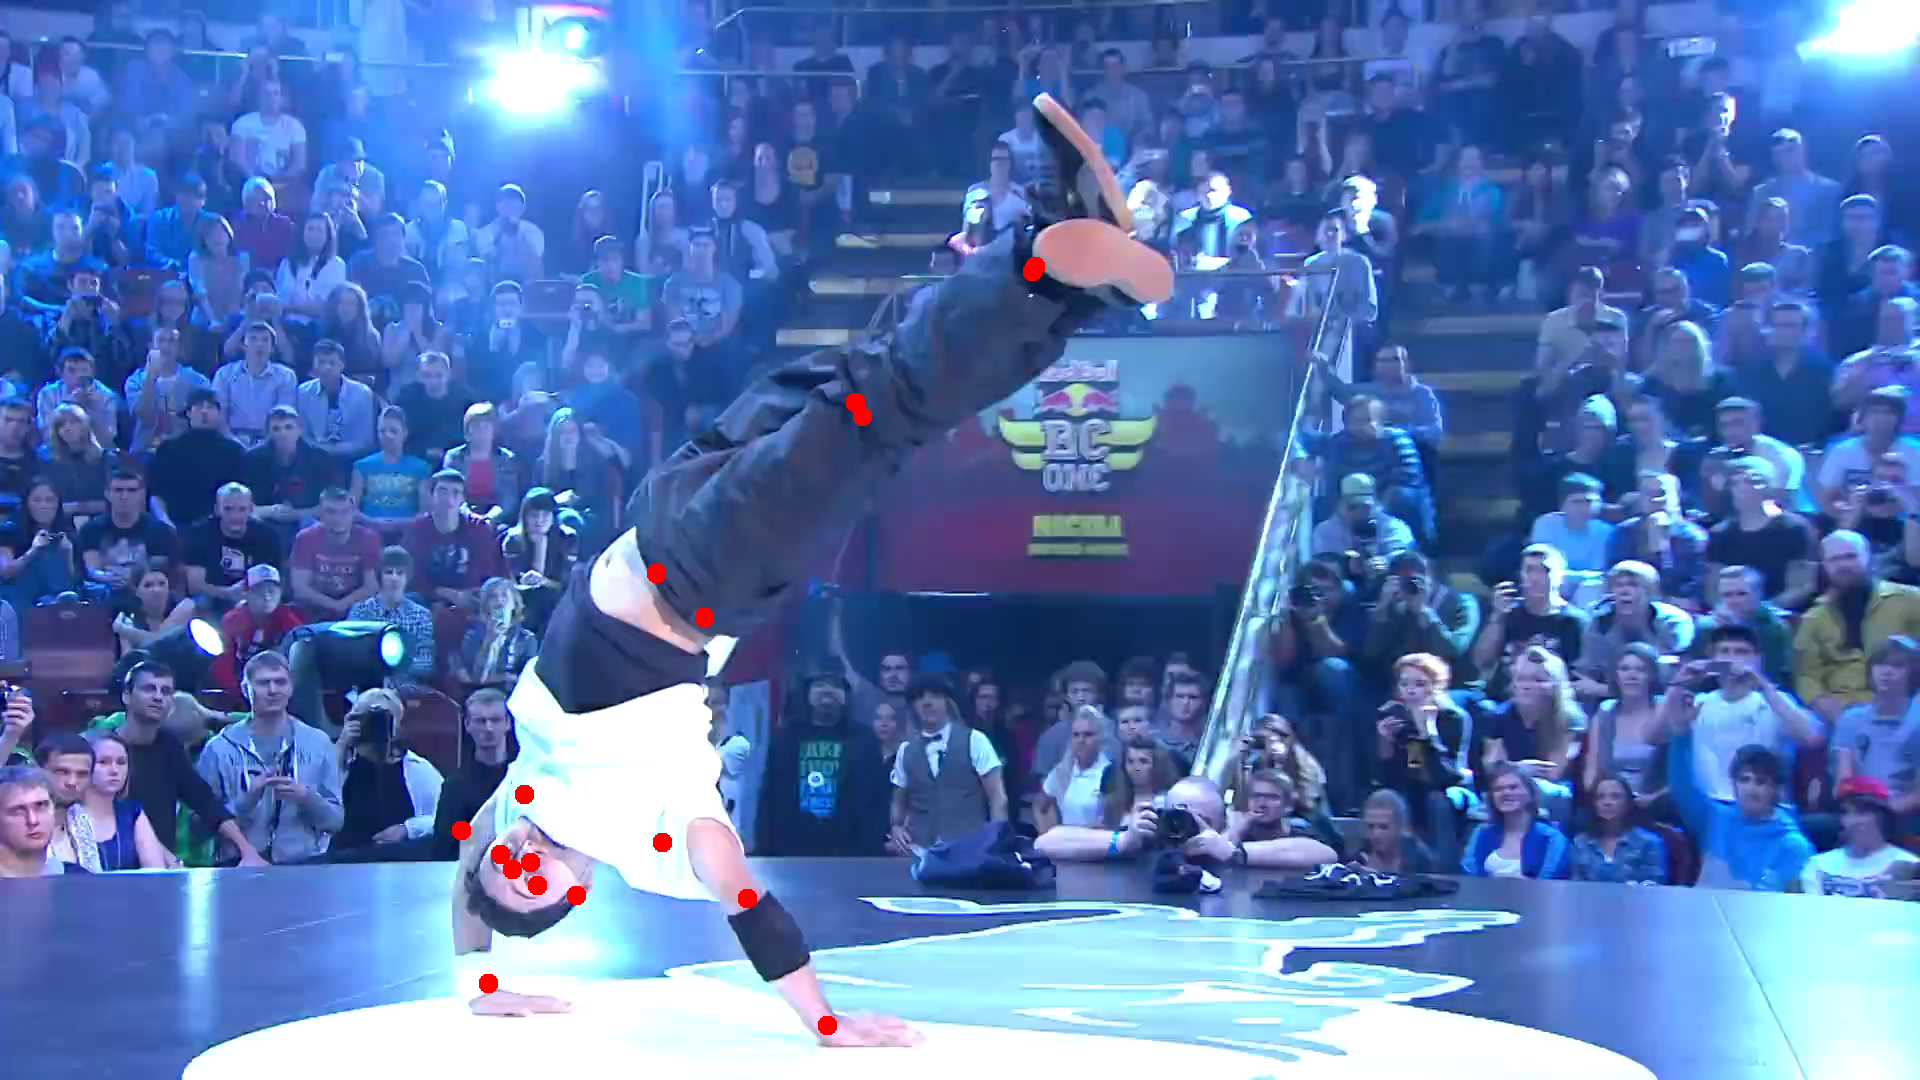
\includegraphics[width=\textwidth]{entities/BRACE_2453.png}
        \caption{Frame 2453}
    \end{subfigure}
    \begin{subfigure}{0.5\textwidth}
        \centering
        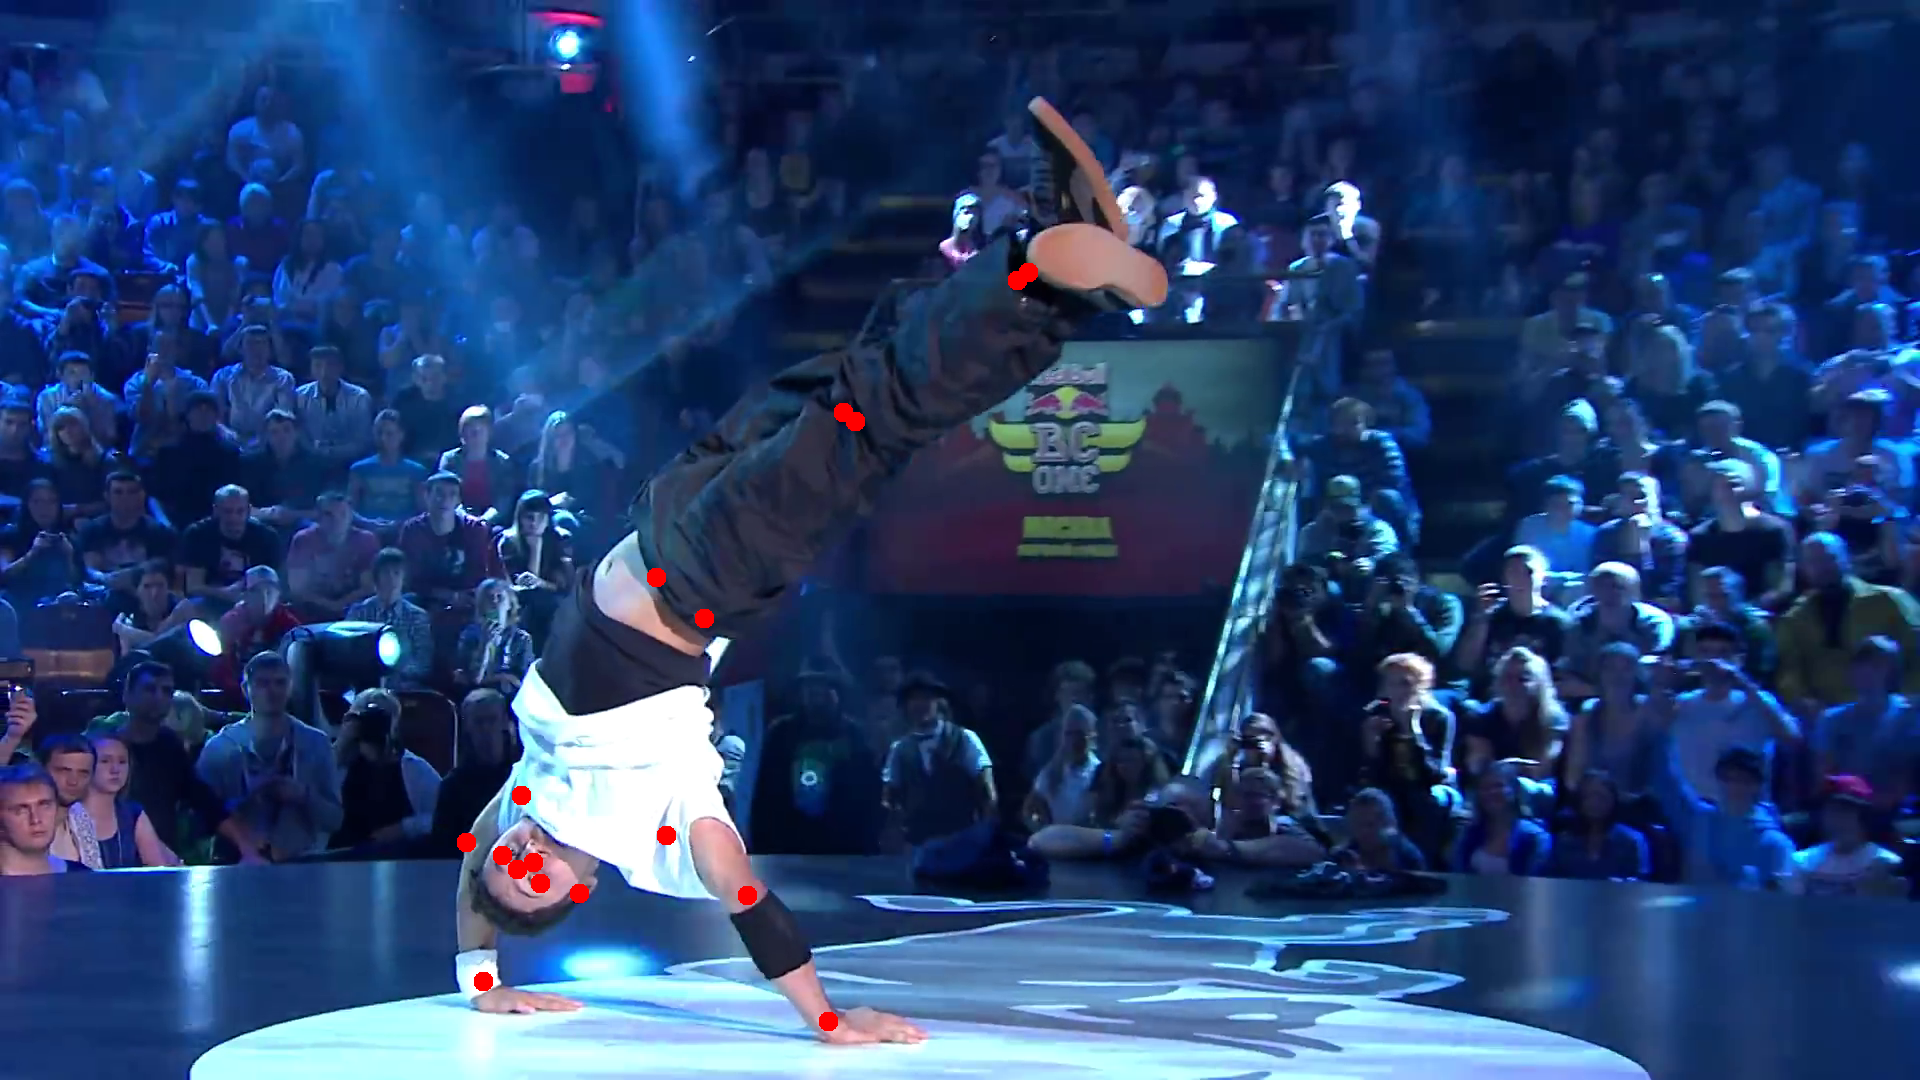
\includegraphics[width=\textwidth]{entities/BRACE_2454.png}
        \caption{Frame 2454}
    \end{subfigure}

    \caption{Example of five consecutive frames of a video from the BRACE-dataset with the corresponding labels,
    where the actor holds his position for a while.}
    \label{fig:BRACE_dataset_static}
\end{figure}

\begin{figure}[htbp]
    \centering
    \begin{subfigure}{0.5\textwidth}
        \centering
        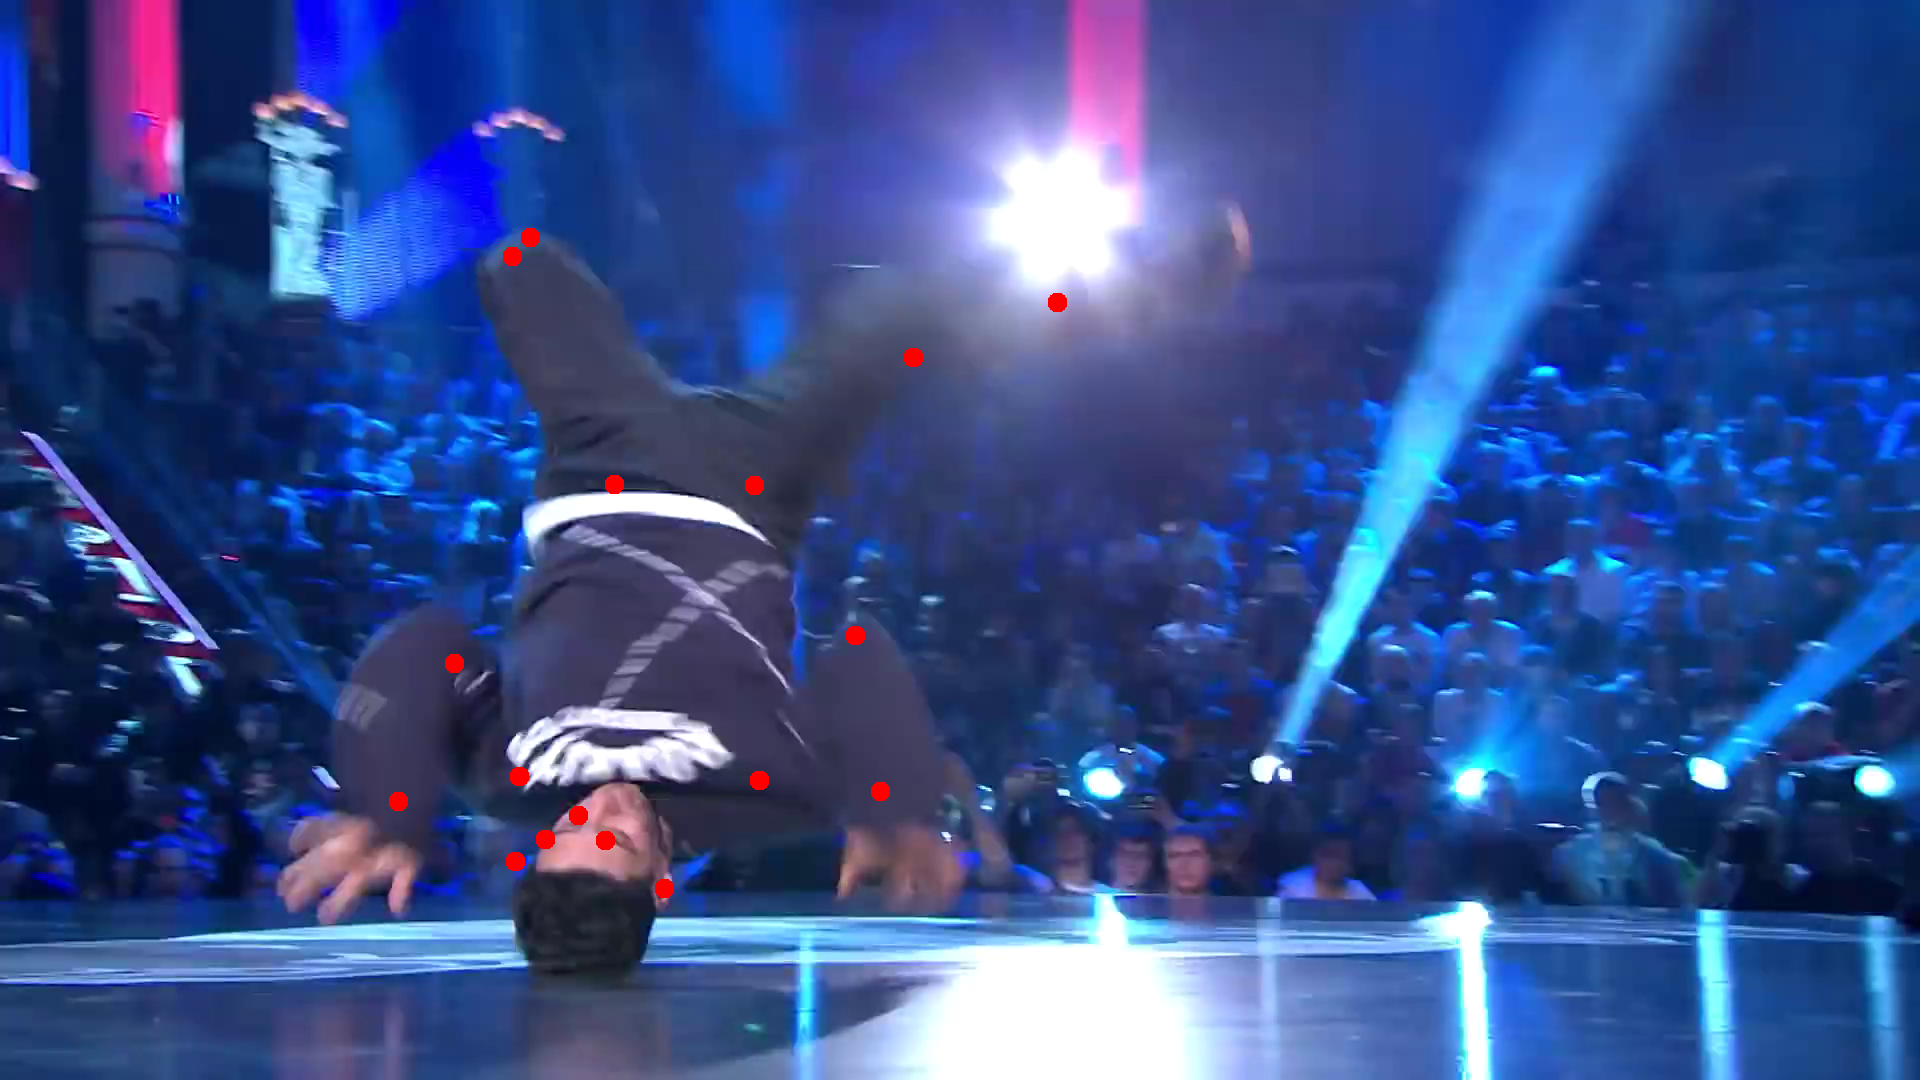
\includegraphics[width=\textwidth]{entities/BRACE_1148.png}
        \caption{Frame 1148}
    \end{subfigure}
    \begin{subfigure}{0.5\textwidth}
        \centering
        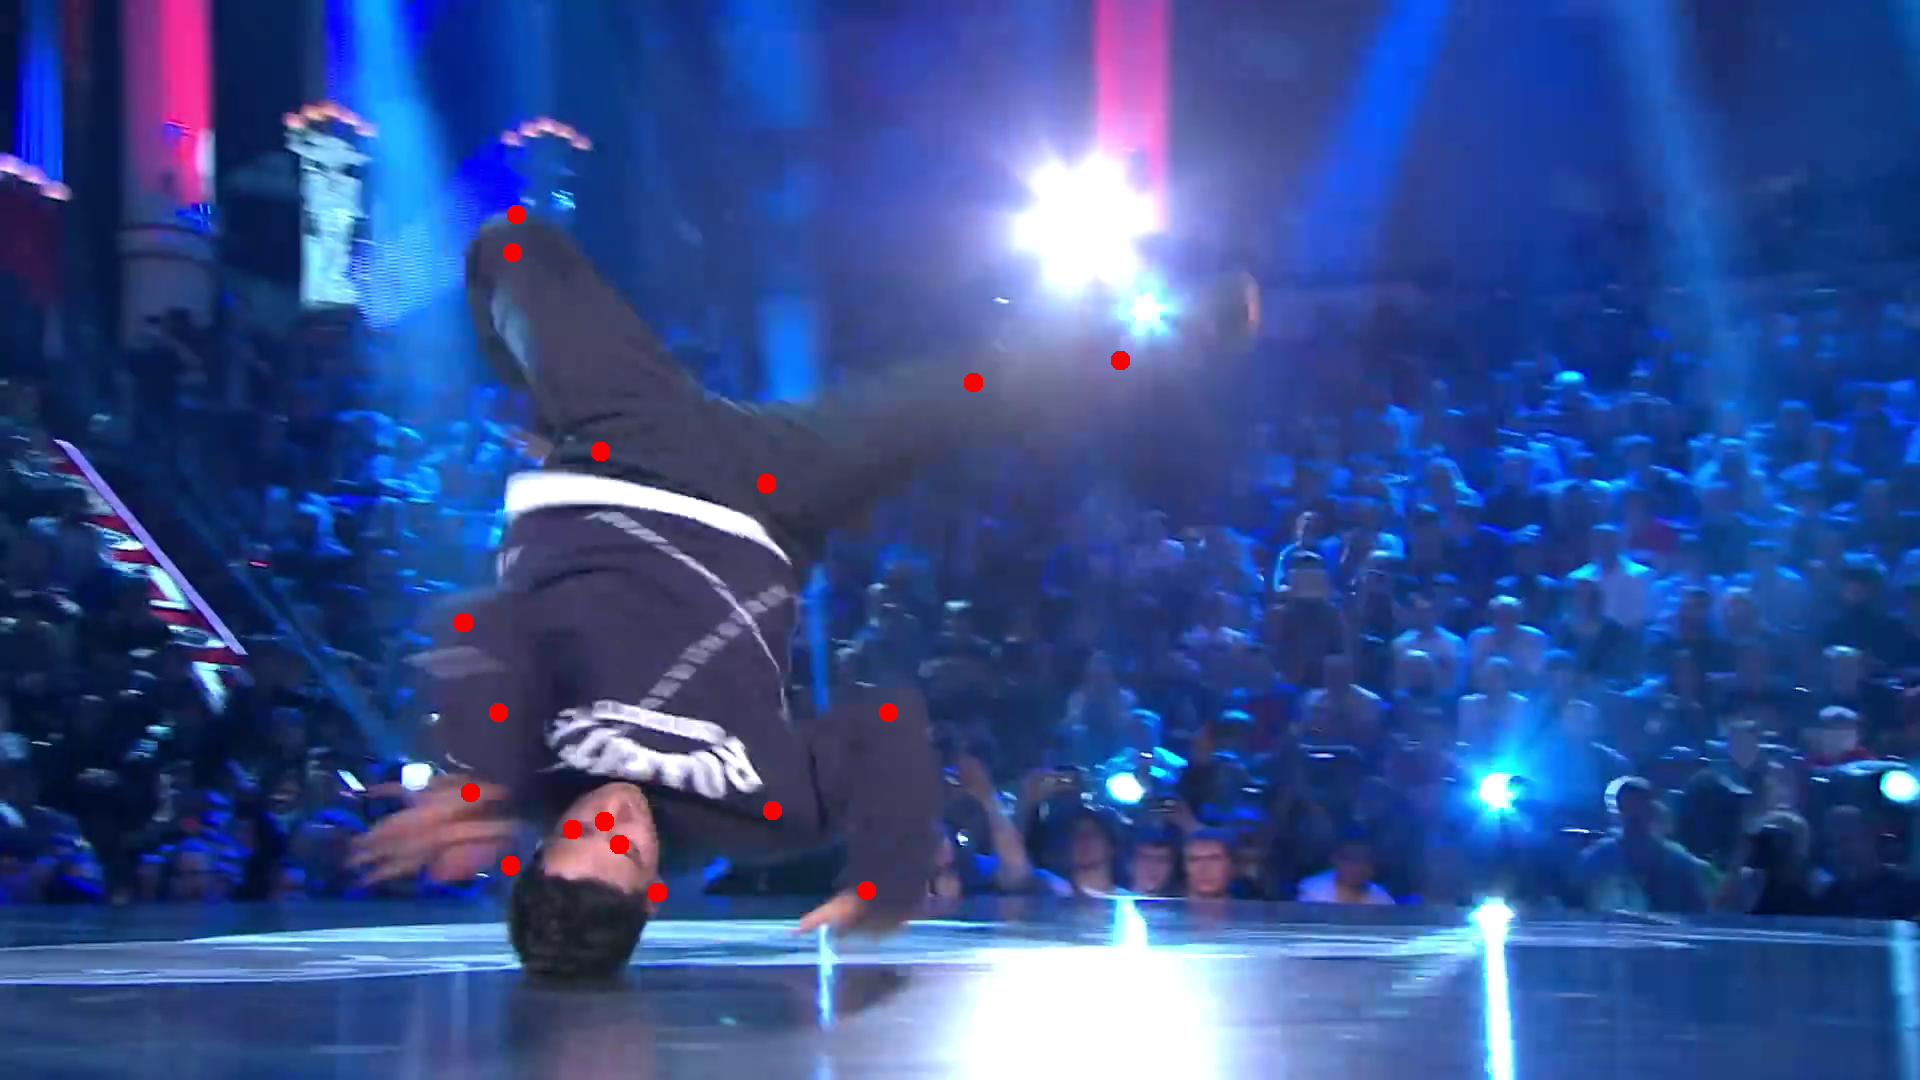
\includegraphics[width=\textwidth]{entities/BRACE_1149.png}
        \caption{Frame 1149}
    \end{subfigure}
    \begin{subfigure}{0.5\textwidth}
        \centering
        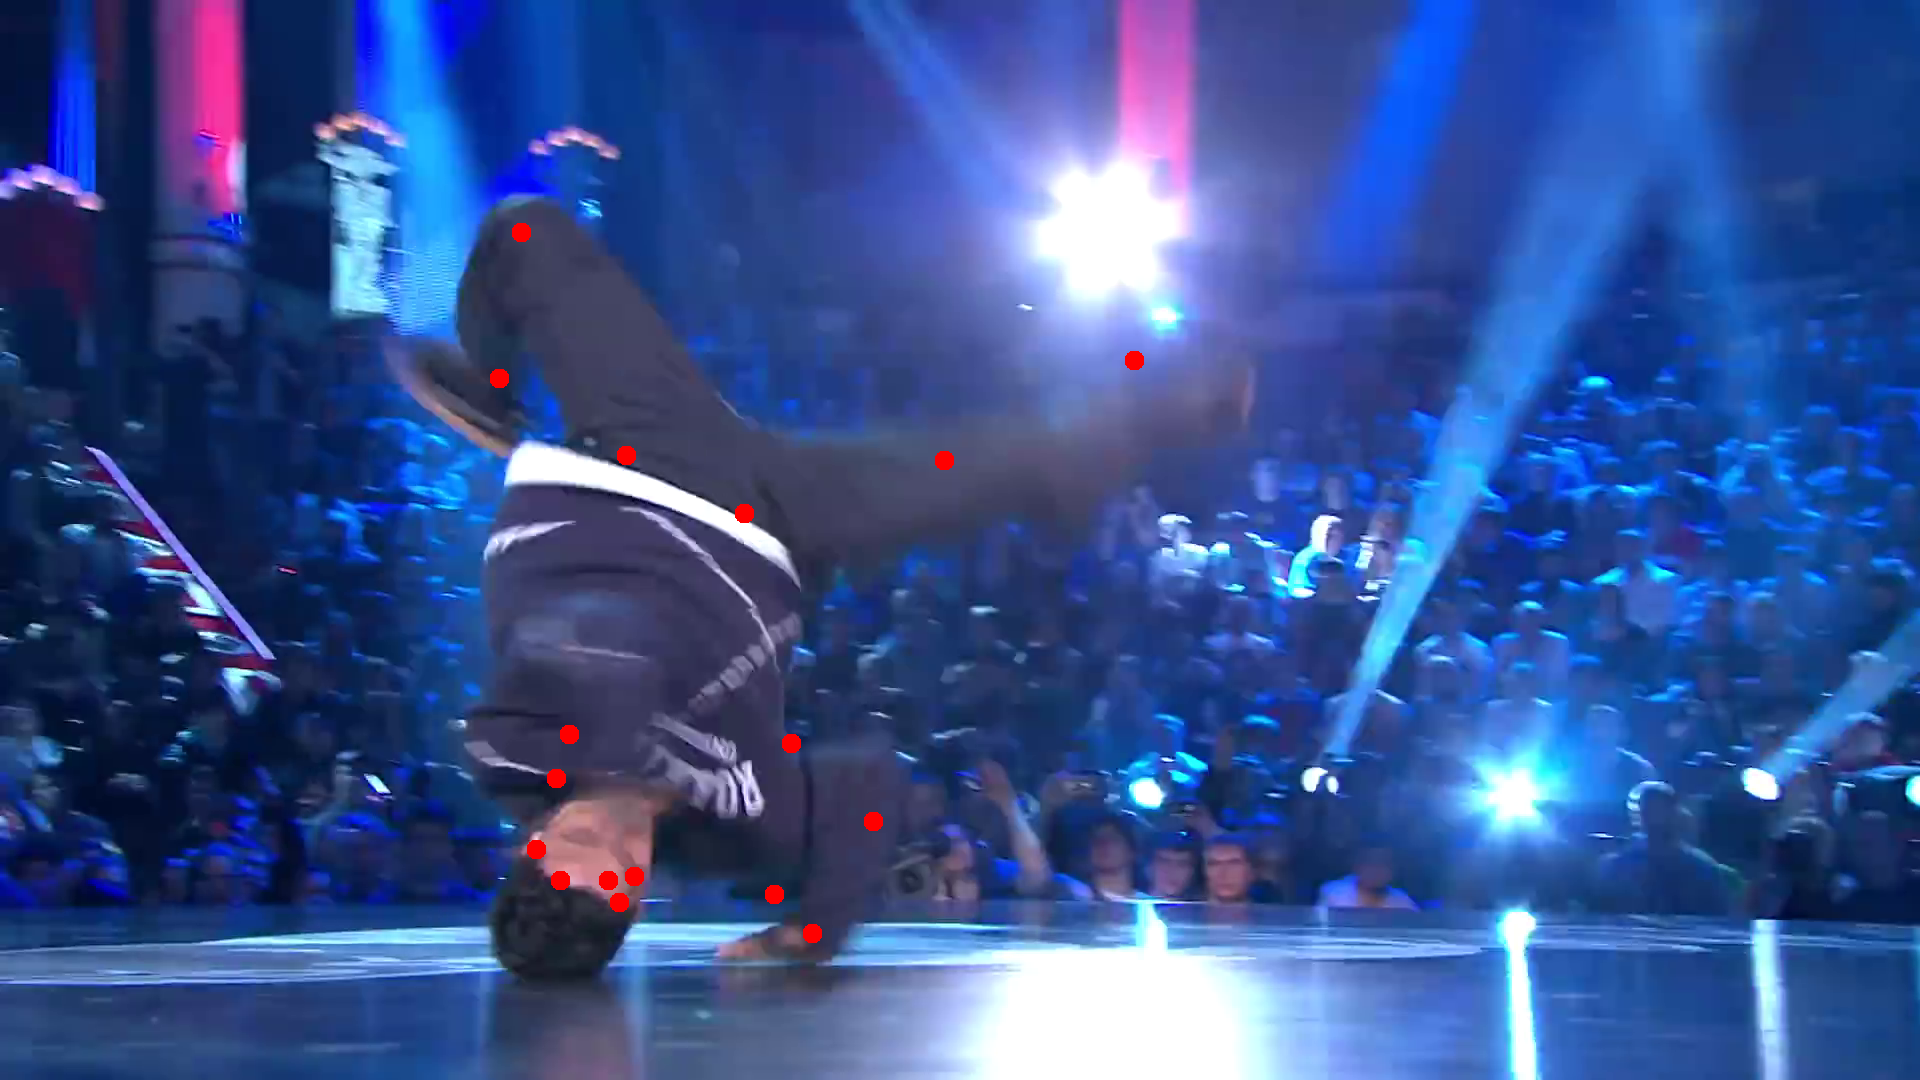
\includegraphics[width=\textwidth]{entities/BRACE_1150.png}
        \caption{Frame 1150}
    \end{subfigure}
    \begin{subfigure}{0.5\textwidth}
        \centering
        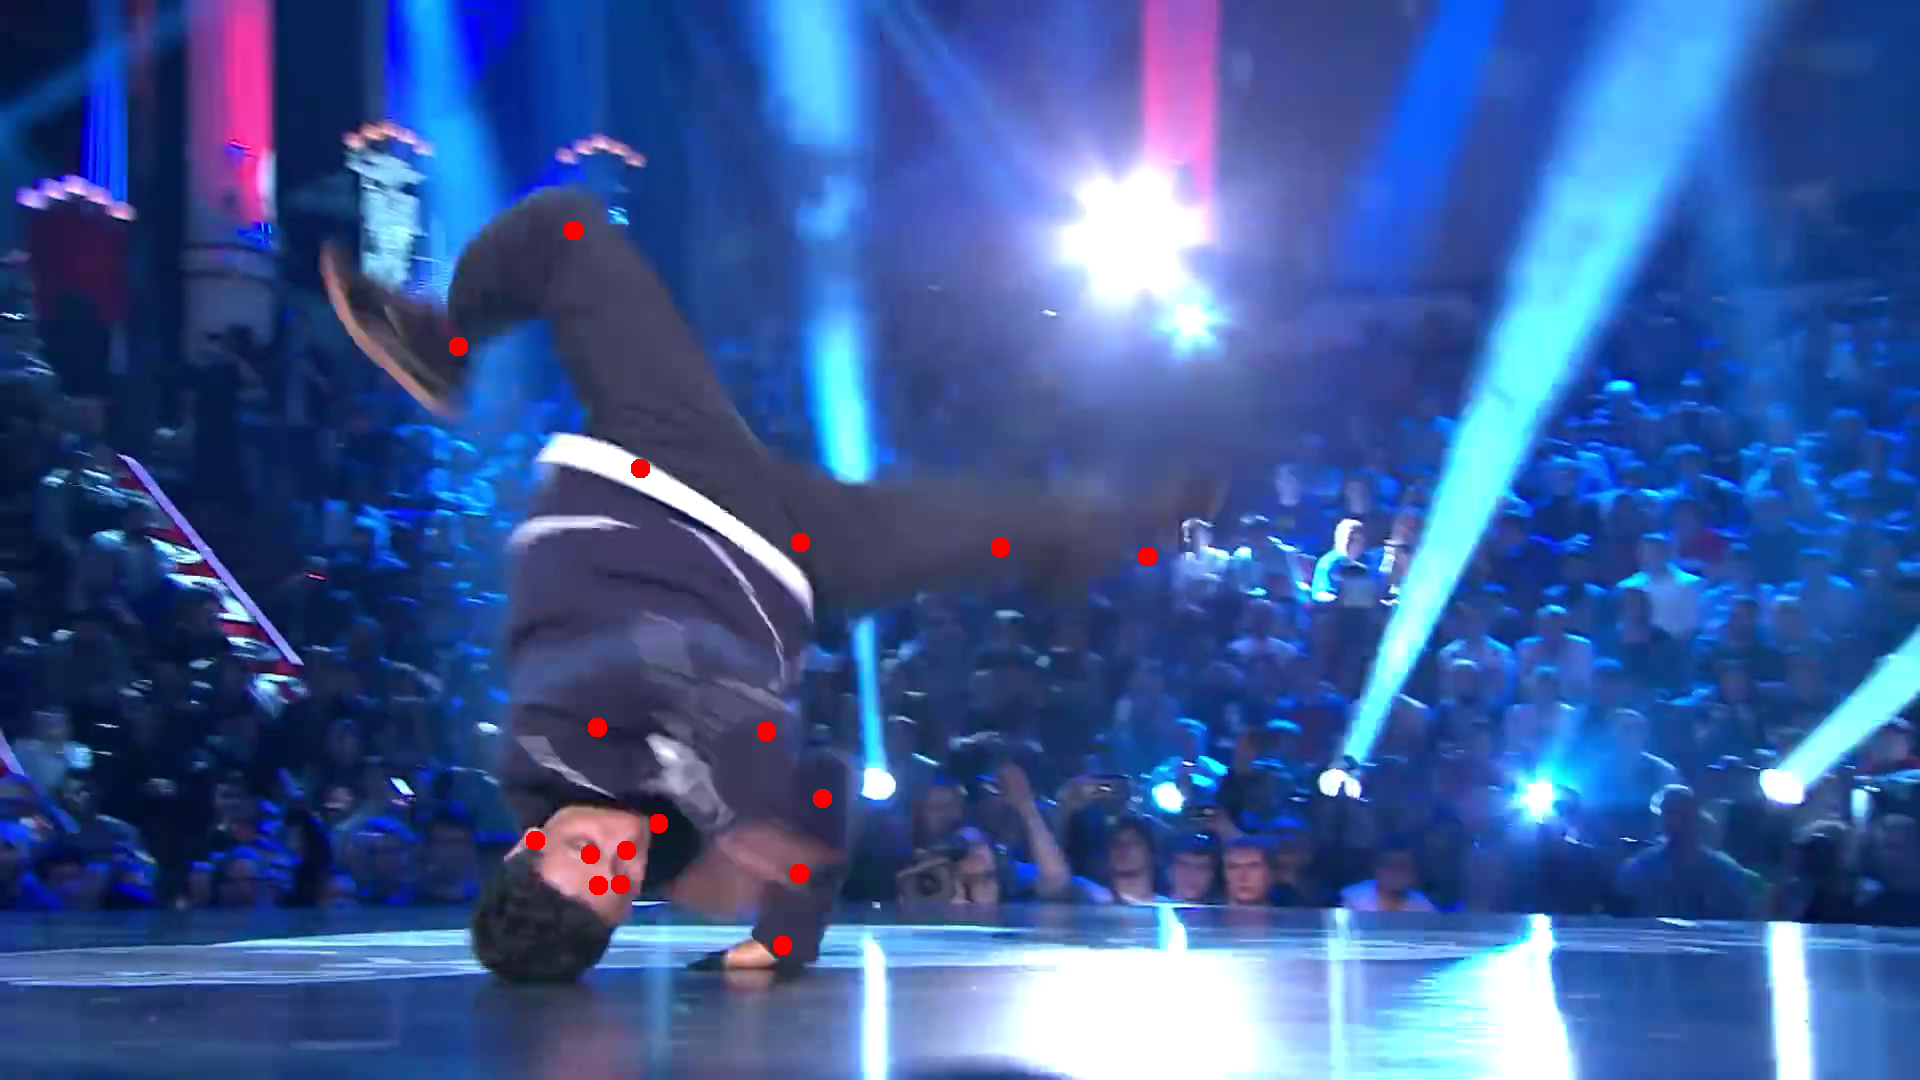
\includegraphics[width=\textwidth]{entities/BRACE_1151.png}
        \caption{Frame 1151}
    \end{subfigure}
    \begin{subfigure}{0.5\textwidth}
        \centering
        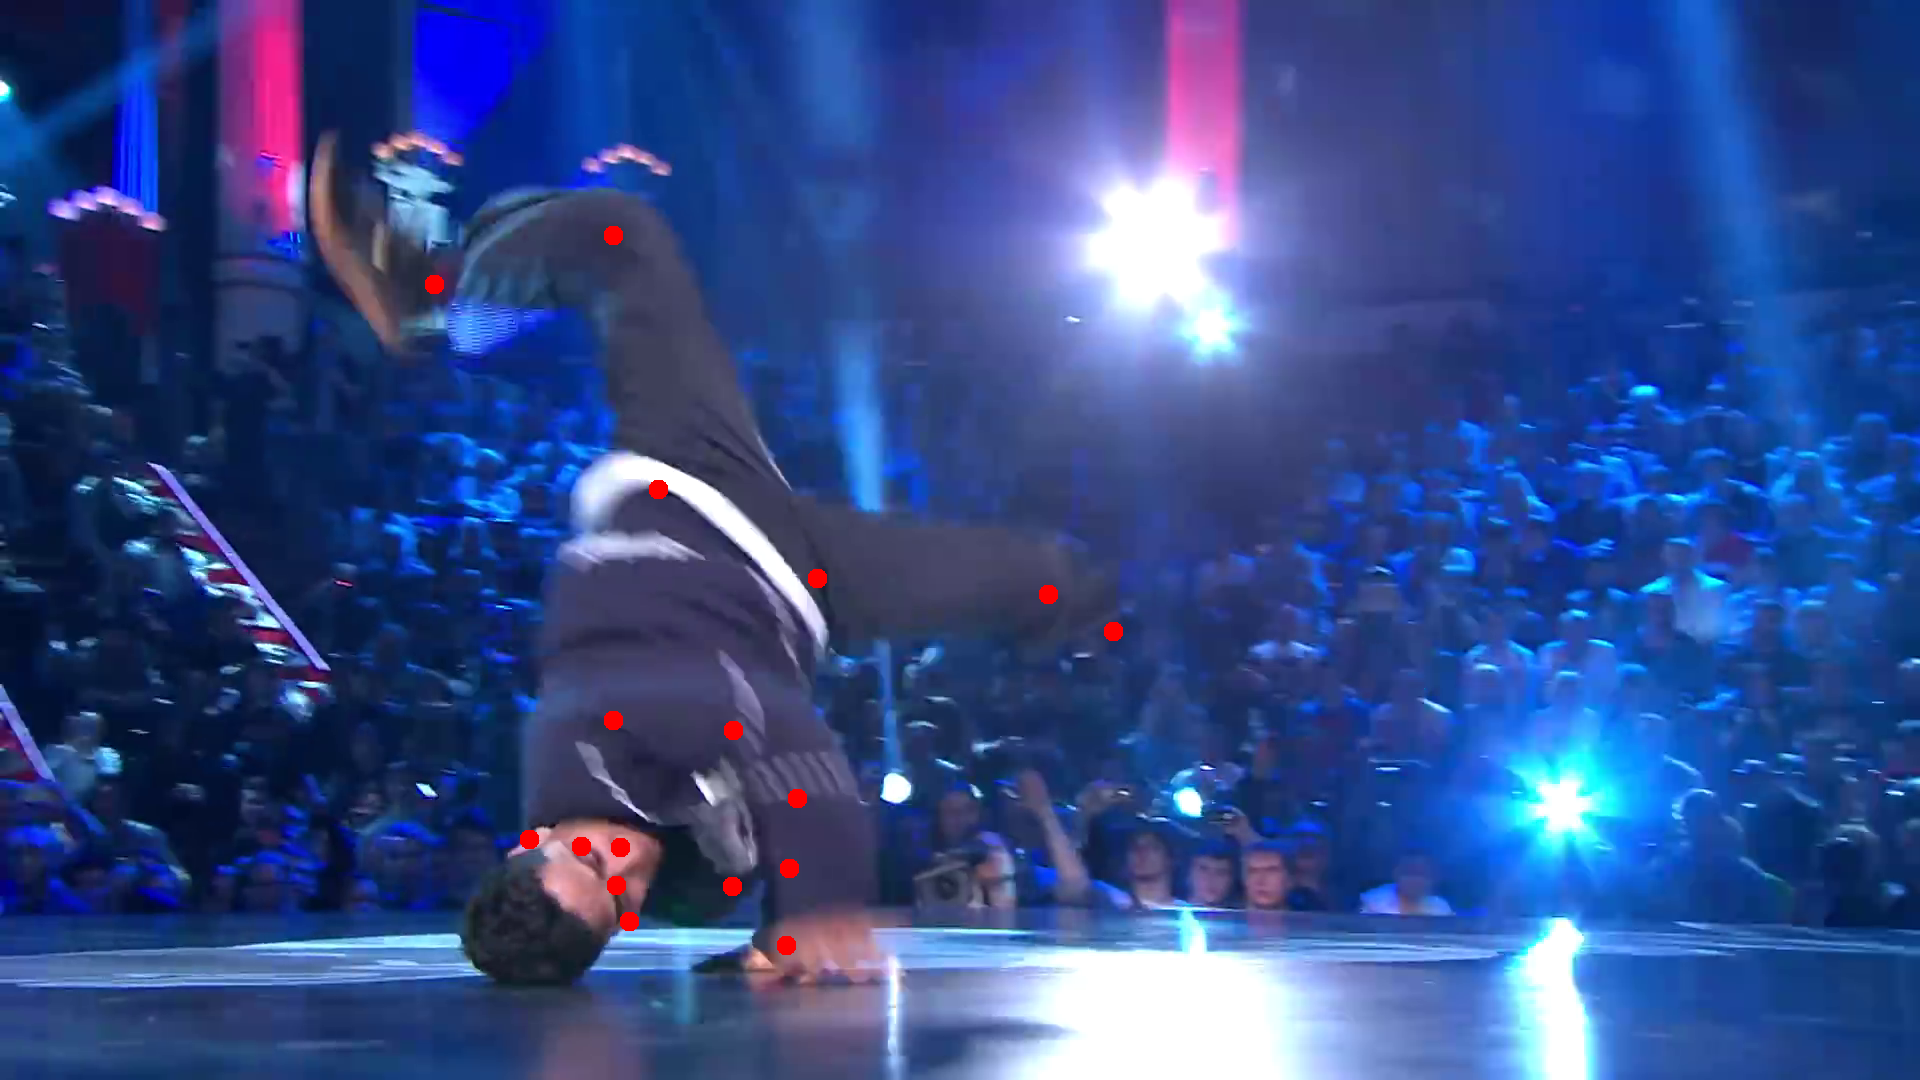
\includegraphics[width=\textwidth]{entities/BRACE_1152.png}
        \caption{Frame 1152}
    \end{subfigure}
    \caption{Example of five consecutive frames of a video from the BRACE-dataset with the corresponding labels, where the actor performs a quick movement.}
    \label{fig:BRACE_dataset_quick}
\end{figure}

\noindent The second dataset we will be using is the \textit{BRACE} dataset \cite{BRACE}. This dataset consists of $1,352$ video sequences and a total of $334,538$ frames with keypoints annotations of breakdancers. The frames of the video sequences have a resolution of $1920 \times 1080$ \cite{BRACE}.
\\
\\
We chose to use this dataset as breakdancers tend to swap between static and quick poses, as well as containing some acrobatic poses, similarly to the ones in the ClimbAlong dataset, making the poses relevant for our experiments in Section \ref{sec:experiments}. Figure \ref{fig:BRACE_dataset_static} and \ref{fig:BRACE_dataset_quick} contains two consecutive sequences, each of five frames, that illustrates these two poses.
\\
\\
The frames of the video sequences have been annotated by initially using state-of-the-art human pose estimators to extract automatic poses. This was then followed by manually annotating bad keypoints, corresponding to difficult poses, as well as pose outliers. Finally, the automatic and manual annotations were merged, interpolating the keypoint seequence with Bézier curves. The keypoints is a list of 17-elements, following the COCO-format, as illustrated in Table \ref{tab:keypoints} \cite{BRACE}.

\subsection{The Penn Action Dataset}
\begin{table}
    \begin{tabular}[htbp]{lllllllllllllll}
        \texttt{baseball\_pitch} & \texttt{baseball\_swing} & \texttt{bench\_press} \\
        \texttt{bowling} & \texttt{clean\_and\_jerk} & \texttt{golf\_swing} \\
        \texttt{jumping\_jacks} & \texttt{jump\_rope} & \texttt{pull\_ups} \\
        \texttt{push\_ups} & \texttt{sit\_ups} & \texttt{squats} \\
        \texttt{strumming\_guitar} & \texttt{tennis\_forehand} & \texttt{tennis\_serve}
    \end{tabular}
    \caption{The original $15$ action-types in the Penn Action dataset.}
    \label{tab:PA_actions}
\end{table}
The final dataset we will be using is the \textit{Penn Action} dataset \cite{penn_action}. This dataset consists of $2326$ video sequences of $15$ different action-types. Table \ref{tab:PA_actions} lists these $15$ action-types \cite{penn_action}.
\\
\\
Each sequence has been manually annotated with human joint annotation, consisting of $13$ joints as well as a corresponding binary visibility-flag for each joint. The frames have a resolution within the size of $640 \times 480$ \cite{penn_action}.
\\
\\
Unlike the BRACE dataset, most of the poses in the Penn Action dataset are not very unusual and thus are not very relevant for the poses of climbers. For that reason, we have decided to focus on the action-types that may contain more unusual poses. Thus, we only keep the sequences that have \texttt{baseball\_pitch}, \texttt{bench\_press} or \texttt{sit\_ups} as their corresponding action-type \cite{penn_action}.
\\
\\
\textbf{HVIS EKSEMPEL}

\subsection{Preprocessing of the Data}
In the following subsections we describe our preprocessing of the various datasets.

\subsubsection{BRACE and Penn Action}
As our models take a sequence of estimated poses as input, and we thus will not be using the images of the videos, we discard the images of all frames from BRACE and Penn Action, such that we only keep the annotated poses.
\\
\\
We start by extracting the bounding-box of the annotated pose in each frame by using the annotated keypoints. Further, we expand each side by $10\%$, such that no keypoint lies on any of the boundaries of the bounding-box. To ensure that the aspect ratio of the pose is kept later on, we transform the bounding-box into a square by extending the shorter sides, such that they have the same length as the longer sides. Next, we discard everything outside the bounding-box and rescale the bounding-box to have a sidelength of $50$, such that it has the same size as the output of the already developed pose-estimator.
\\
\\
Next, we transform each sample into twenty five heatmaps. This is done by creating twenty five $50 \times 50$ zero-matrices for each sample, such that each zero-matrix represents a single keypoint of a single sample. Further, for each keypoint we insert a $1$ at the position of the keypoint in its corresponding zero-matrix and apply a Gaussian filter with mean $\mu = 0$ and standard deviation $\sigma = 1$ to smear out each heatmap. For missing keypoints, we do not place a $1$ in the corresponding heatmap, making the heatmap consist of only zeros. Further, as Penn Action is the only dataset with the position of the head annotated, as well as the only dataset missing a annotation for the nose, we treat the head-annotation of Penn Action as if it was a nose-annotation, as the position of the two annotation would be very close to each other.
\\
\\
The heatmaps that we produce by following the above description will be used as the groundtruth output of our models. However, as we will be pretraining our models detached from the already developed pose-estimator, we will also need some data as input. We acquire this data by introducing some noise to the data, such that they become similar to the output of the already developed pose-estimator, essentially simulating the output of the already developed pose-estimator. The noise is introduced by randomly shifting each keypoint of each sample and by smearing our each keypoint of each sample by using a Gaussian filter, where the standard deviation is randomly chosen. For the shift-value, we $2.62$, as this is approximately equal to $0.2x$ where $x$ is the mean torso-diameter. We clip the new position of each keypoint between $0$ and $49$, such that the position of the new keypoint cannot be outside the heatmap. For the random standard deviation we sample uniformly at random from the set $\{1, 1.5, 2, 2.5, 3\}$.

\subsubsection{ClimbAlong}


\end{document}